% Options for packages loaded elsewhere
\PassOptionsToPackage{unicode}{hyperref}
\PassOptionsToPackage{hyphens}{url}
%
\documentclass[
  english,
  man]{apa6}
\usepackage{lmodern}
\usepackage{amssymb,amsmath}
\usepackage{ifxetex,ifluatex}
\ifnum 0\ifxetex 1\fi\ifluatex 1\fi=0 % if pdftex
  \usepackage[T1]{fontenc}
  \usepackage[utf8]{inputenc}
  \usepackage{textcomp} % provide euro and other symbols
\else % if luatex or xetex
  \usepackage{unicode-math}
  \defaultfontfeatures{Scale=MatchLowercase}
  \defaultfontfeatures[\rmfamily]{Ligatures=TeX,Scale=1}
\fi
% Use upquote if available, for straight quotes in verbatim environments
\IfFileExists{upquote.sty}{\usepackage{upquote}}{}
\IfFileExists{microtype.sty}{% use microtype if available
  \usepackage[]{microtype}
  \UseMicrotypeSet[protrusion]{basicmath} % disable protrusion for tt fonts
}{}
\makeatletter
\@ifundefined{KOMAClassName}{% if non-KOMA class
  \IfFileExists{parskip.sty}{%
    \usepackage{parskip}
  }{% else
    \setlength{\parindent}{0pt}
    \setlength{\parskip}{6pt plus 2pt minus 1pt}}
}{% if KOMA class
  \KOMAoptions{parskip=half}}
\makeatother
\usepackage{xcolor}
\IfFileExists{xurl.sty}{\usepackage{xurl}}{} % add URL line breaks if available
\IfFileExists{bookmark.sty}{\usepackage{bookmark}}{\usepackage{hyperref}}
\hypersetup{
  hidelinks,
  pdfcreator={LaTeX via pandoc}}
\urlstyle{same} % disable monospaced font for URLs
\usepackage{graphicx,grffile}
\makeatletter
\def\maxwidth{\ifdim\Gin@nat@width>\linewidth\linewidth\else\Gin@nat@width\fi}
\def\maxheight{\ifdim\Gin@nat@height>\textheight\textheight\else\Gin@nat@height\fi}
\makeatother
% Scale images if necessary, so that they will not overflow the page
% margins by default, and it is still possible to overwrite the defaults
% using explicit options in \includegraphics[width, height, ...]{}
\setkeys{Gin}{width=\maxwidth,height=\maxheight,keepaspectratio}
% Set default figure placement to htbp
\makeatletter
\def\fps@figure{htbp}
\makeatother
\setlength{\emergencystretch}{3em} % prevent overfull lines
\providecommand{\tightlist}{%
  \setlength{\itemsep}{0pt}\setlength{\parskip}{0pt}}
\setcounter{secnumdepth}{-\maxdimen} % remove section numbering
% Make \paragraph and \subparagraph free-standing
\ifx\paragraph\undefined\else
  \let\oldparagraph\paragraph
  \renewcommand{\paragraph}[1]{\oldparagraph{#1}\mbox{}}
\fi
\ifx\subparagraph\undefined\else
  \let\oldsubparagraph\subparagraph
  \renewcommand{\subparagraph}[1]{\oldsubparagraph{#1}\mbox{}}
\fi
% Manuscript styling
\usepackage{upgreek}
\captionsetup{font=singlespacing,justification=justified}

% Table formatting
\usepackage{longtable}
\usepackage{lscape}
% \usepackage[counterclockwise]{rotating}   % Landscape page setup for large tables
\usepackage{multirow}		% Table styling
\usepackage{tabularx}		% Control Column width
\usepackage[flushleft]{threeparttable}	% Allows for three part tables with a specified notes section
\usepackage{threeparttablex}            % Lets threeparttable work with longtable

% Create new environments so endfloat can handle them
% \newenvironment{ltable}
%   {\begin{landscape}\begin{center}\begin{threeparttable}}
%   {\end{threeparttable}\end{center}\end{landscape}}
\newenvironment{lltable}{\begin{landscape}\begin{center}\begin{ThreePartTable}}{\end{ThreePartTable}\end{center}\end{landscape}}

% Enables adjusting longtable caption width to table width
% Solution found at http://golatex.de/longtable-mit-caption-so-breit-wie-die-tabelle-t15767.html
\makeatletter
\newcommand\LastLTentrywidth{1em}
\newlength\longtablewidth
\setlength{\longtablewidth}{1in}
\newcommand{\getlongtablewidth}{\begingroup \ifcsname LT@\roman{LT@tables}\endcsname \global\longtablewidth=0pt \renewcommand{\LT@entry}[2]{\global\advance\longtablewidth by ##2\relax\gdef\LastLTentrywidth{##2}}\@nameuse{LT@\roman{LT@tables}} \fi \endgroup}

% \setlength{\parindent}{0.5in}
% \setlength{\parskip}{0pt plus 0pt minus 0pt}

% Overwrite redefinition of paragraph and subparagraph by the default LaTeX template
% See https://github.com/crsh/papaja/issues/292
\makeatletter
\renewcommand{\paragraph}{\@startsection{paragraph}{4}{\parindent}%
  {0\baselineskip \@plus 0.2ex \@minus 0.2ex}%
  {-1em}%
  {\normalfont\normalsize\bfseries\itshape\typesectitle}}

\renewcommand{\subparagraph}[1]{\@startsection{subparagraph}{5}{1em}%
  {0\baselineskip \@plus 0.2ex \@minus 0.2ex}%
  {-\z@\relax}%
  {\normalfont\normalsize\itshape\hspace{\parindent}{#1}\textit{\addperi}}{\relax}}
\makeatother

% \usepackage{etoolbox}
\makeatletter
\patchcmd{\HyOrg@maketitle}
  {\section{\normalfont\normalsize\abstractname}}
  {\section*{\normalfont\normalsize\abstractname}}
  {}{\typeout{Failed to patch abstract.}}
\patchcmd{\HyOrg@maketitle}
  {\section{\protect\normalfont{\@title}}}
  {\section*{\protect\normalfont{\@title}}}
  {}{\typeout{Failed to patch title.}}
\makeatother
\shorttitle{SHORTTITLE}
\usepackage{csquotes}
\usepackage{float}
\usepackage{sectsty}
\usepackage{lscape}
\newcommand{\blandscape}{\begin{landscape}}
\newcommand{\elandscape}{\end{landscape}}
\ifxetex
  % Load polyglossia as late as possible: uses bidi with RTL langages (e.g. Hebrew, Arabic)
  \usepackage{polyglossia}
  \setmainlanguage[]{english}
\else
  \usepackage[shorthands=off,main=english]{babel}
\fi

\author{\phantom{0}}
\date{}


\affiliation{\phantom{0}}

\begin{document}

\hypertarget{chapitre-5-les-tests-duxe9quivalence}{%
\section{Chapitre 5: les tests d'équivalence}\label{chapitre-5-les-tests-duxe9quivalence}}

Lorsqu'on applique un test d'hypothèse, l'hypothèse nulle la plus couramment définie est celle d'absence d'effet ou de différence entre les groupes ({\textbf{???}}). Il arrive également parfois que les chercheurs définissent un intervalle de valeur comme hypothèse nulle, mais le plus souvent, cet intervalle est borné par la valeur 0 ({\textbf{???}}), on parle alors d'hypothèse unilatérale. Avec cette stratégie, le rejet de l'hypothèse nulle constitue un soutien en faveur de la présence d'un effet non nul. Par contre, le non rejet de l'hypothèse nulle ne peut être interprété comme un soutien en faveur de l'absence d'effet, or il arrive souvent que des chercheurs l'interprètent de la sorte. ({\textbf{???}}), par exemple, ont reporté que parmis 150 articles publiés entre 1940 et 1999 dans le \emph{JAP} (\emph{Journal of Applied Psychology}), 38\% interprétaient un résultat non significatif comme une acceptation de l'hypothès nulle. Plus récemment, ({\textbf{???}}) a noté que l'expression \enquote{pas d'effet} a été utilisée dans 108 articles publié dans \emph{Social Psychological and Personality Science} avant août 2016 et que dans presque tous les cas, c'était sur base du non rejet de l'hypothèse nulle que cette conclusion était tirée.

A travers ce chapitre, notre premier objectif sera d'expliquer pourquoi interpréter le non rejet de l'hypothèse d'absence d'effet comme un soutien en faveur d'une absence d'effet n'est pas une bonne stratégie. Nous introduirons ensuite les tests d'équivalence qui permettent d'obtenir un soutien en faveur d'un effet jugé non pertinent, et plus particulièrement le TOST (Two One-sided test). Pour finir, nous présenterons un article dans lequel nous comparons le TOST à la \emph{SGPV} (Second Generation P-value), une stratégie récemment développée par ({\textbf{???}}).

\hypertarget{limites-de-lapproche-traditionnelle}{%
\subsection{Limites de l'approche traditionnelle}\label{limites-de-lapproche-traditionnelle}}

Lorsqu'on teste une hypothèse nulle, il y a deux conclusions possibles: soit ont la rejette soit on ne la rejette pas. Si rejeter l'hypothèse nulle amène à conclure en faveur de l'hypothèse alternative, ne pas la rejeter ne permet pas de conclure en faveur de l'hypothèse nulle. Au mieux, cela nous montre que les données ne sont pas incompatibles avec l'hypothèse nulle, mais cela ne veut en aucun cas dire qu'elles ne sont compatibles avec aucune autre hypothèse. Afin de l'illustrer, la Table 1 résume les résultats de simulations Monte Carlo pour un ensemble de 70 scénarios qui varient en fonction de la taille des échantillons (\(n_j\)) et de la différence entre les moyennes des deux populations dont sont extraits les échantillons (\(\mu_1-\mu_2\)). Pour chaque scénario, à 5000 reprises, nous avons généré une paire d'échantillons, réalisé un test \(t\) de Student pour échantillons indépendants et extrait la \(p\)-valeur du test. Ensuite, nous avons calculé la proportion de \(p\)-valeurs supérieures à .05 (le risque alpha communément accepté, {\textbf{???}}), nous amenant à ne pas rejeter l'hypothèse nulle. Cette proportion correspond au taux d'erreur de type II (communément appelé \(\beta\)).

\begin{center}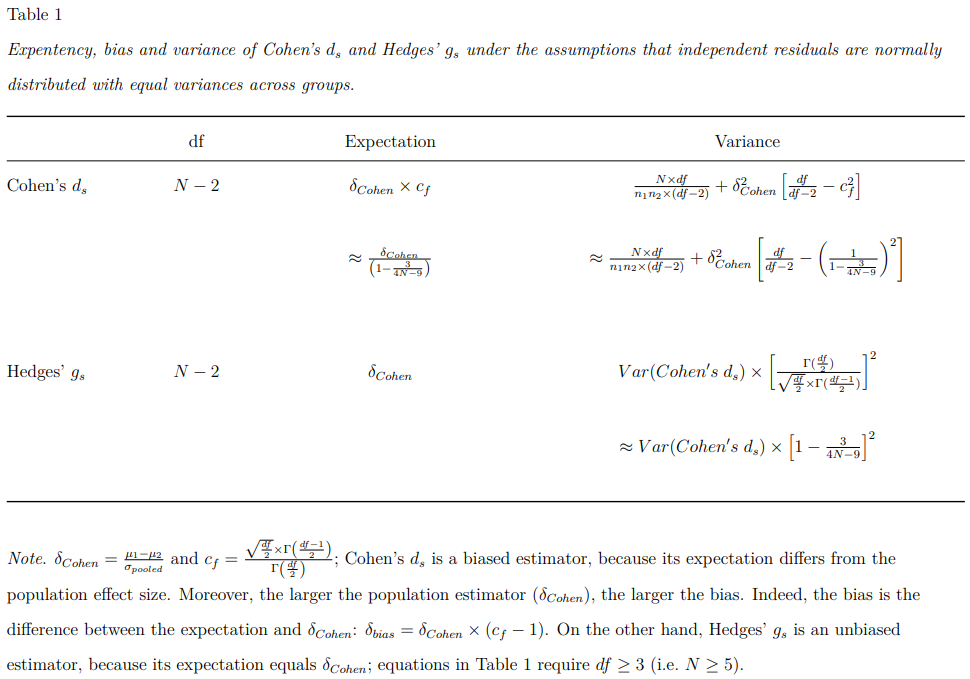
\includegraphics[width=0.96\linewidth]{D:/Documents/Github_projects/thesis/Chapitre 5/Illustration/Table 1} \end{center}

Dans la mesure où une vraie différence entre les moyennes de population existe pour l'ensemble des scénarios envisagés, nous espérerions être en mesure de rejeter l'hypothèse nulle le plus souvent possible. Pourtant, pour plusieurs scénarios, le nombre d'itérations amenant à conclure au non rejet de l'hypothèse nul est bien supérieur au nombre d'itérations amenant à conclure au rejet de l'hypothèse nulle, comme on peut le voir à travers les valeurs \(\beta\) très élevées dans certains cas. Par exemple, avec 10 sujets par groupes et considérant \(\sigma_1=\sigma_2=1\), on ne détectera pas une différence de moyenne de .1 dans près de 95\% des cas. Avec 200 sujets par groupe, on ne détectera toujours pas cette différence dans 80\% des cas. En présence d'un effet non nul, cela se justifie par un manque de puissance des tests réalisés, ce qui démontre bien qu'un non rejet de l'hypothèse nulle peut en fait signifier deux choses: soit qu'il n'y a vraiment pas de différence entre les moyennes des populations (ou autrement dit, que les différences observées sont dûes au hasard), soit que le test n'est pas suffisamment puissant pour détecter la différence. Or, le manque de puissance des tests est récurrent dans la littérature, comme tendent à le montrer diverses méta-analyses (voir par exemple {\textbf{???}}; {\textbf{???}}; {\textbf{???}}).

Pour éviter d'interpréter un test peu puissant comme un soutien en faveur de l'hypothèse nulle, dans les années 80, l'approche de la puissance est devenue l'approche par défaut pour tester l'équivalence ({\textbf{???}}). A travers cette approche qui est restée très populaire ({\textbf{???}}), dans un premier temps, on définit ce qu'on considère comme étant la plus petite valeur d'intérêt (en anglais, le \enquote{SESOI} pour \enquote{Smaller Effect Size of Interest}), c'est-à-dire la taille d'effet minimale requise pour considérer qu'un effet est pertinent. Ensuite, on estime la puissance de notre test à détecter un effet de cette taille\footnote{On parle d'estimation et non de mesure, car la puissance dépend de paramètres de population qu'on ne connait pas (Schuirmann,1987).}, et si cette estimation atteind une valeur jugée satisfaisante (en général, 80\%), alors on considère que l'on peut interpréter le non rejet de l'hypothèse nulle d'absence d'effet comme soutien en faveur de l'équivalence ({\textbf{???}}; {\textbf{???}}; {\textbf{???}}). L'idée sous-jacente est que si l'effet est au moins aussi grand que les limites de la zone d'équivalence, on devrait rejeter l'hypothèse nulle dans un pourcentage raisonnable de cas. Par conséquent, un non rejet de l'hypothèse nulle devrait vraisemblablement signifier que l'effet n'atteint pas le SESOI et donc, que l'effet observé n'est pas pertinent.

\begin{verbatim}
## pdf 
##   2
\end{verbatim}

Bien que ce raisonnement puisse sembler tentant, de prime abord, il présente d'importantes limites. Via cette approche, la probabilité de détecter une absence d'effet va augmenter non seulement quand la taille des échantillons va diminuer (à condition de ne pas passer en deça de la puissance minimale requise), mais également quand l'erreur (la variabilité des scores au sein de chaque groupe) va augmenter ({\textbf{???}}; {\textbf{???}}). Ce dernier point est illustré au sein de la Figure \ref{fig:schuirman}. Sur l'axe des abscisses, on représente différentes estimations de la différence de moyenne (\(\bar{X_1}-\bar{X_2}\)) et sur l'axe des ordonnées, la précision des estimations \(\bar{X_1}-\bar{X_2}\) (\(S\sqrt{\frac{2}{n}}\) correspond à l'estimation l'erreur standard de \(\bar{X_1}-\bar{X_2}\), avec \(S\) étant l'écart-type poolé et \(n\) la taille de chaque échantillon, lorsque les échantillons ont tous les deux la même taille et sont extraits de population ayant la même variance)\footnote{Par facilité, à l'instar de Schuirman (1987), on envisage le cas où les échantillons sont de même taille et que l'on suppose que la condition d'homogénéité des variances est respectée. Notons cependant que d'après Schuirman, ce raisonnement peut être généralisé aux scénarios où les deux échantillons n'ont pas la même taille et sont extraits de population n'ayant pas la même variance.}. Le triangle grisé représente l'ensemble des combinaisons estimation/précision qui vont amener à conclure à l'équivalence, avec l'approche de la puissance, lorsqu'on travaille avec des échantillons de taille 50, en acceptant un risque \(\alpha\) de 5\% et en exigeant une puissance minimale de 80\% pour détecter une différence de 20 unités (\(|\theta_j=20| (j=1,2)\)). Pour toutes les valeurs de \(S\sqrt{\frac{2}{n}}\) supérieures à 7.07 aucune estimation de différence de moyennes ne permettra de conclure à l'équivalence (pas même 0) puisque la puissance du test classique est inférieure à 80. Pour toutes les valeurs de \(S\sqrt{\frac{2}{n}}\) inférieures à 7.07, on constate que plus notre estimation de \(\bar{X_1}-\bar{X_2}\) est précise (lorsqu'on se déplace du haut vers le bas, sur l'axe des ordonnées), plus l'estimation doit être proche de 0 pour pouvoir conclure à l'équivalence. Ce n'est bien entendu pas une propriété désirable ({\textbf{???}}).

\begin{figure}

{\centering 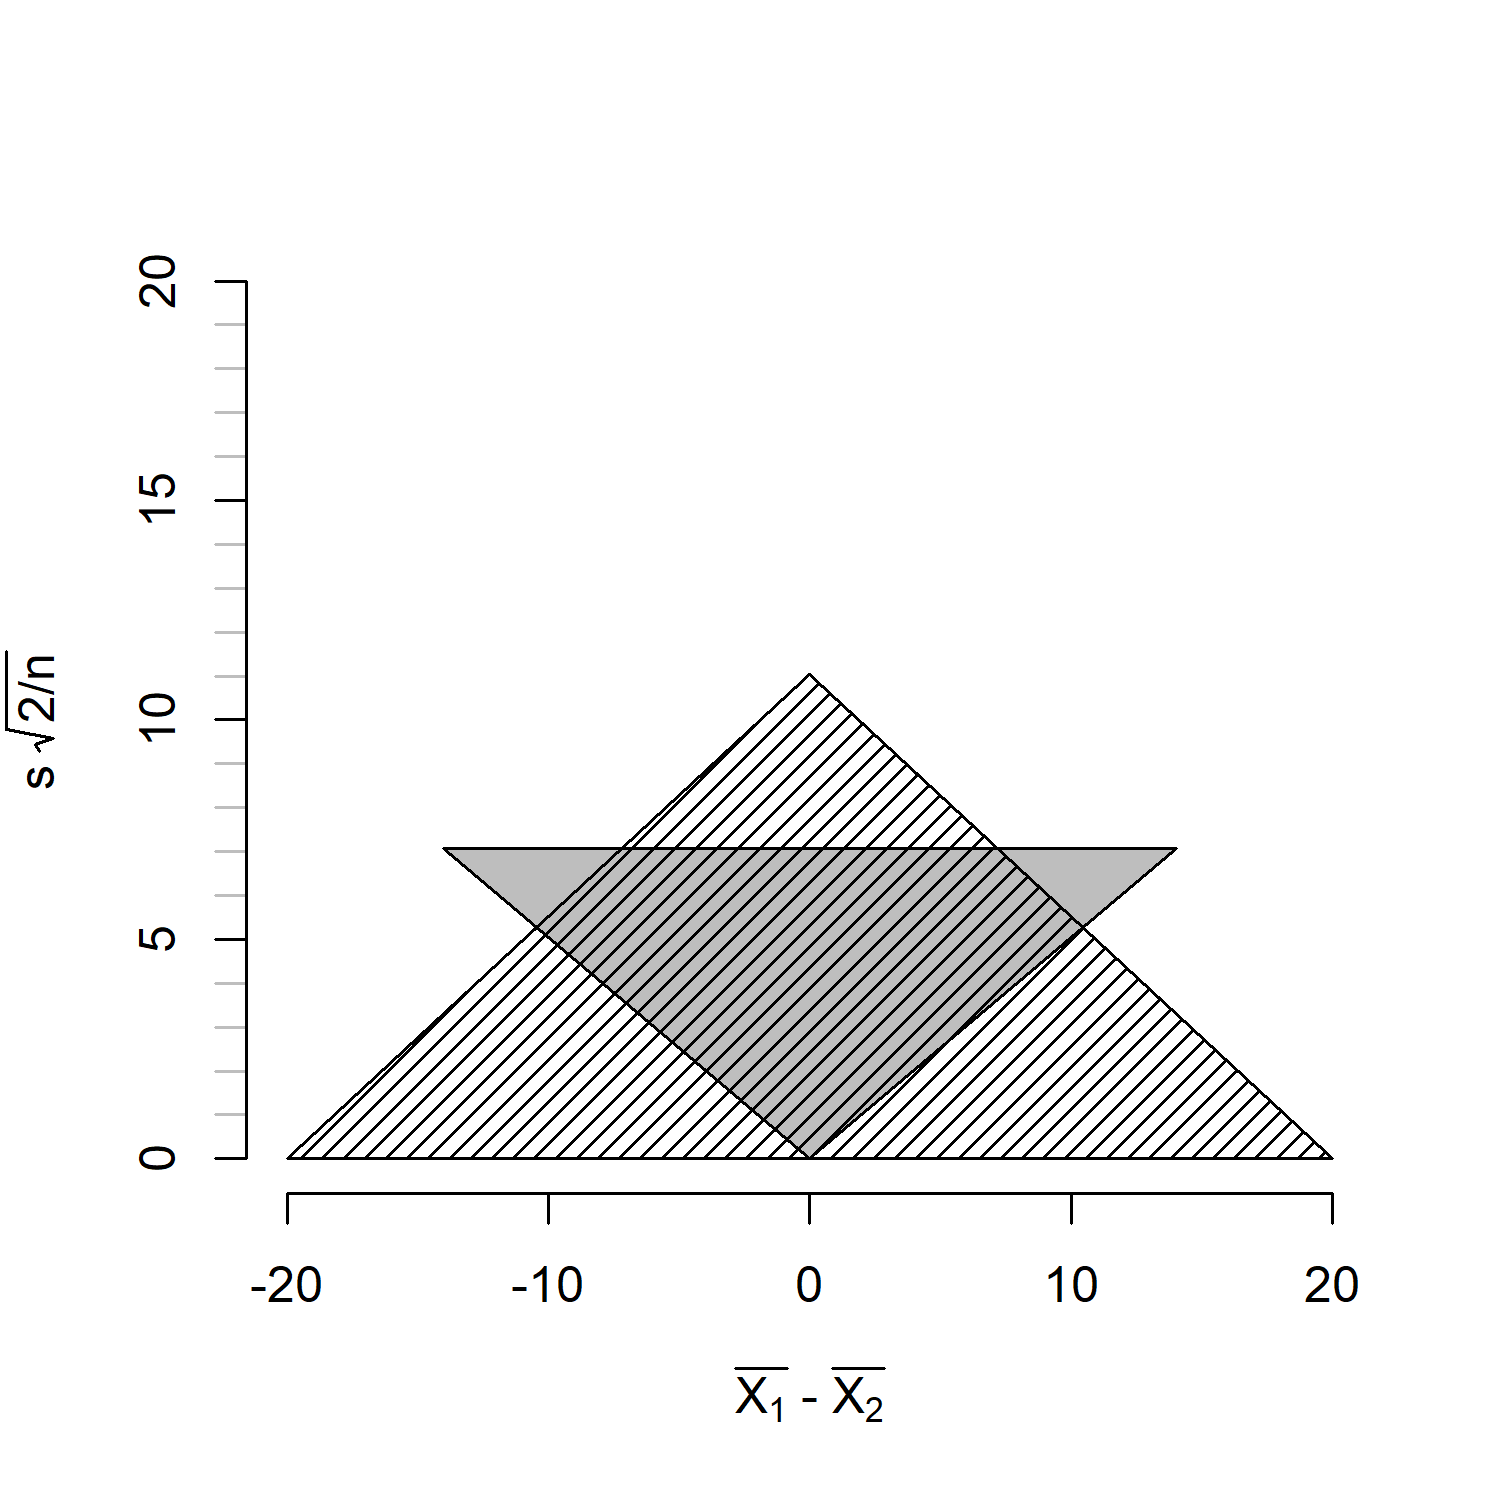
\includegraphics[width=0.96\linewidth]{D:/Documents/Github_projects/thesis/Chapitre 5/Illustration/Fig1} 

}

\caption{Région d'équivalence pour l'approche de la puissance (zone grisée) et pour le TOST (zone hachurée), pour l'exemple où $|\theta$|=20, n = 50 et $\alpha=.05$}\label{fig:schuirman2}
\end{figure}

\hypertarget{les-tests-duxe9quivalence}{%
\subsection{Les tests d'équivalence}\label{les-tests-duxe9quivalence}}

Avec les tests d'équivalence, il n'est pas possible de démontrer qu'un effet vaille exactement zéro ({\textbf{???}}). Il est par contre possible de montrer que l'effet observé est suffisamment petit pour être jugé non pertinent. Le point de départ des tests d'équivalence est de définir \(\theta_1\) et \(\theta_2\), les limites inférieures et supérieures de la zone d'équivalence, cette dernière contenant l'ensemble des valeurs jugées trop petites pour être susceptibles de nous intéresser. Ces limites peuvent être exprimées soit dans l'unité des données brutes, soit en terme standardisé.

Il existe ensuite plusieurs approches pour démontrer que l'effet observé se situe ans la zone d'équivalence (\emph{voir Meyners, par exemple}). Parmis celles-ci, une approche très simple est celle du \emph{TOST} (pour \enquote{Two one-sided tests}, ({\textbf{???}}); ({\textbf{???}}))\footnote{il existe des alternatives au TOST qui sont très légèrement plus puissantes, mais le gain marginal en termes de puissance est contrebalancé par un niveau de complexité beaucoup plus élevé (Meyners, 2012).}. Le principe est de définir deux hypothèses nulles: la première est que l'effet observé est inférieur à la limite inférieure de la zone d'équivalence: \[H0_1: \theta < \theta_1\] La deuxième est que l'effet observé est supérieur à la limite supérieure de la zone d'équivalence: \[H0_2: \theta > \theta_2\] Lorsque les deux hypothèses nulle peuvent être simultanément rejetées, on peut conclure à l'équivalence (Seaman \& Serlin, 1998, cités par lakens\_equivalence\_2017). Il est à noter qu'il n'est pas nécessaire de réaliser deux tests pour rejeter les deux hypothèse nulles. En effet, si l'effet observé se situe à équidistance des deux limites de la zone d'équivalence, les tests contre chacune des limites mèneront à une conclusion identique, car ils seront associés à la même valeur de statistique (en termes absolu) et par conséquent seront associés à la même \(p\)-valeur. Si l'effet observé ne se situe \emph{pas} à égale distance des deux limites de la zone d'équivalence, alors il suffira de tester l'hypothèse nulle qui se rapporte à la limite la plus proche de l'effet observé. En effet, le test associé à cette limite sera nécessairement celui qui est associé à la plus petite valeur de statistique et donc, à la plus grande \(p\)-valeur ({\textbf{???}}).

A titre d'illustration, la Figure \ref{fig:equiv1} montre\ldots{} (expliquer la figure: le carré = diff de moyenne observée, etc.)

\begin{figure}

{\centering 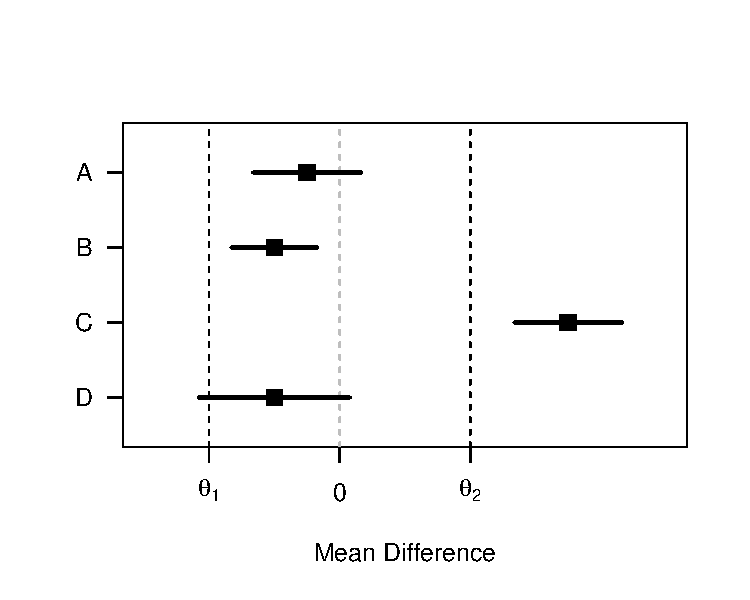
\includegraphics{chp5_files/figure-latex/equiv1-1} 

}

\caption{Différence de moyennes ($\bar{X_1}-\bar{X_2}$), distribution d'échantillonnage et IC à $1-2\alpha\%$ autour de la différence de moyennes ($\bar{X_1}-\bar{X_2}$) pour 3 exemples de TOST.}\label{fig:equiv1}
\end{figure}

Statistiquement parlant, montrer que les deux hypothèses nulles peuvent être rejetées, en considérant un risque \(\alpha\) donné, équivaut à montrer que l'intervalle de confiance à \((1-2\times\alpha)\%\) est entièrement inclus dans la zone d'équivalence ({\textbf{???}}). L'avantage de l'approche par intervalles de confiance est que ces derniers peuvent généralement être calculés dans la plupart des logiciels statistiques, contrairement aux tests d'équivalence qui ne sont pas encore disponibles partout ({\textbf{???}}).

\hypertarget{avantage-des-tests-duxe9quivalence}{%
\subsection{Avantage des tests d'équivalence}\label{avantage-des-tests-duxe9quivalence}}

On ne peut falsifier une théorie si elle ne prédit pas une taille d'effet. Si elle ne le fait pas, même si on ne parvient pas à répliquer un effet signifiatif, on pourrait encore argumenter qu'il y a bien un effet mais plus petit que ce que l'étude était capable de détecter (Morey \& Lakens, 2017, cités par {\textbf{???}}).

\hypertarget{conclusions-possibles}{%
\subsection{Conclusions possibles}\label{conclusions-possibles}}

\begin{enumerate}
\def\labelenumi{\arabic{enumi})}
\tightlist
\item
  statistical indeterminacy ({\textbf{???}})
\item
  equivalence ({\textbf{???}})
\end{enumerate}

Lorsqu'ils sont combinés avec un test traditionnel pour lequel l'hypothèse nulle est l'absence d'effet, les TOST peuvent amener à 4 conclusions distinctes:
1) Equivalent et non statistiquement différent de 0: on conclura à l'absence de différence ayant un intérêt pratique ({\textbf{???}}).
2) Statistiquement différent de 0, mais équivalent: il existe un effet non nul, mais trop petit pour avoir un intérêt. C'est ce qui peut typiquement arriver avec des échantillons trop larges (résultant en des tests \enquote{trop}puissants, ({\textbf{???}}))\\
3) Statistiquement différent de 0, et on ne peut conclure à l'équivalence: on conclura alors à la présence d'un effet ({\textbf{???}})
4) Ni statistiquement différent de 0 ni équivalent (quand les données sont si imprécises qu'on ne peut rien tirer comme conclusion)\\
--\textgreater{} A illustrer quand Jamovi le voudra!

\hypertarget{duxe9finir-les-limites-de-la-zone-duxe9quivalencele-sesoi}{%
\subsection{Définir les limites de la zone d'équivalence:LE sesoi}\label{duxe9finir-les-limites-de-la-zone-duxe9quivalencele-sesoi}}

L'aspect le plus compliqué dans la réalisation du TOST est la définition des bornes d'équivalence. Il existe plusieurs stratégies:\\
1) définir comme limites la plus petite taille d'effet pour laquelle on peut atteindre une puissance de détection suffisante (déterminé par les ressources disponibles pour étudier l'effet, ({\textbf{???}})) --\textgreater{} voir la section \enquote{Setting equivalence bounds} p.~359 mais je crois que j'en parle aussi dans la vidéo SOCLAB.\\
2) le SESOI peut parfois être fixé objectivement
3) Idéalement basé sur une analyse coût-bénéfice). Attention: bien sûr une dimension subjective dans la définition des coûts et des bénéfices.
Attention: le SESOI doit être déterminé AVANT et INDEPENDAMMENT des données.

\hypertarget{les-4-conclusions-possibles-quand-combinuxe9-au-nhst-classique}{%
\subsection{Les 4 conclusions possibles quand combiné au NHST classique}\label{les-4-conclusions-possibles-quand-combinuxe9-au-nhst-classique}}

Voir ({\textbf{???}}) p.~357. J'en parle ou po?

\hypertarget{morceau-qui-servira-peut-uxeatre-ou-pas}{%
\subsection{Morceau qui servira peut-être (ou pas)}\label{morceau-qui-servira-peut-uxeatre-ou-pas}}

D'après ({\textbf{???}}), un test d'hypothèse (selon l'approche de Nayman-Pearson) vaut la peine à 2 conditions:\\
1) que l'hypothèse nulle soit assez plausible pour que son rejet puisse surprendre au moins certains;\\
2) le chercheur veut appliquer une procédure méthodol qui l'autorise à prendre des décisions quant à la manière d'agir, tout en contrôlant le taux d'erreur. Agir peut vouloir dire: adopter un traitement, une politique, une intervention, ou abandonner un domaine de rechercher, modifier une manipulation, ou de faire un certain type de déclaration ou revendication.\\
*One of the most widely suggested improvements of the use of p values is to replace null-ypothesis tests (where the goal is to reject ann effect of exactly 0) with tests of range predictions (where the goal is to reject effects that fall outside of the range of effects that is predicted or considered practically important) ({\textbf{???}}).

Un autre argument en défaveur de la p-valeur est la tendance des chercheurs à interpréter un effet NS comme l'acceptation de l'hypothèse nulle (Schmidt, 1996, cité par Harris, 1997). Une fois encore, l'usage des tailles d'effet peut aider à cette fin, non pas en \enquote{remplaçant} les tests d'hypothèses, mais en les complétant. --\textgreater{} Tests d'équivalence.

\hypertarget{remarques-diverses}{%
\subsection{Remarques diverses}\label{remarques-diverses}}

D'après Meyners, il existe pleins d'approches mais la différence entre elles est souvent négligeable ({\textbf{???}}).

\hypertarget{quand-veut-on-montrer-une-absence-deffet}{%
\subsection{Quand veut-on montrer une absence d'effet?}\label{quand-veut-on-montrer-une-absence-deffet}}

Il arrive que des chercheurs souhaitent obtenir un soutien en faveur d'une absence d'effet. A titre d'illustration, ({\textbf{???}}) évoquent la situation où un chercheur désire écarter de potentielles covariables de leur analyse, en démontrant préalablement que ces variables ne sont pas corrélées à la variable dépendante. ESSAYER DE TROUVER ENCORE UN EXEMPLE. Or, on constate que très souvent,
- Pour justifier la décision de pooler plusieurs groupes ({\textbf{???}}).

\begin{center}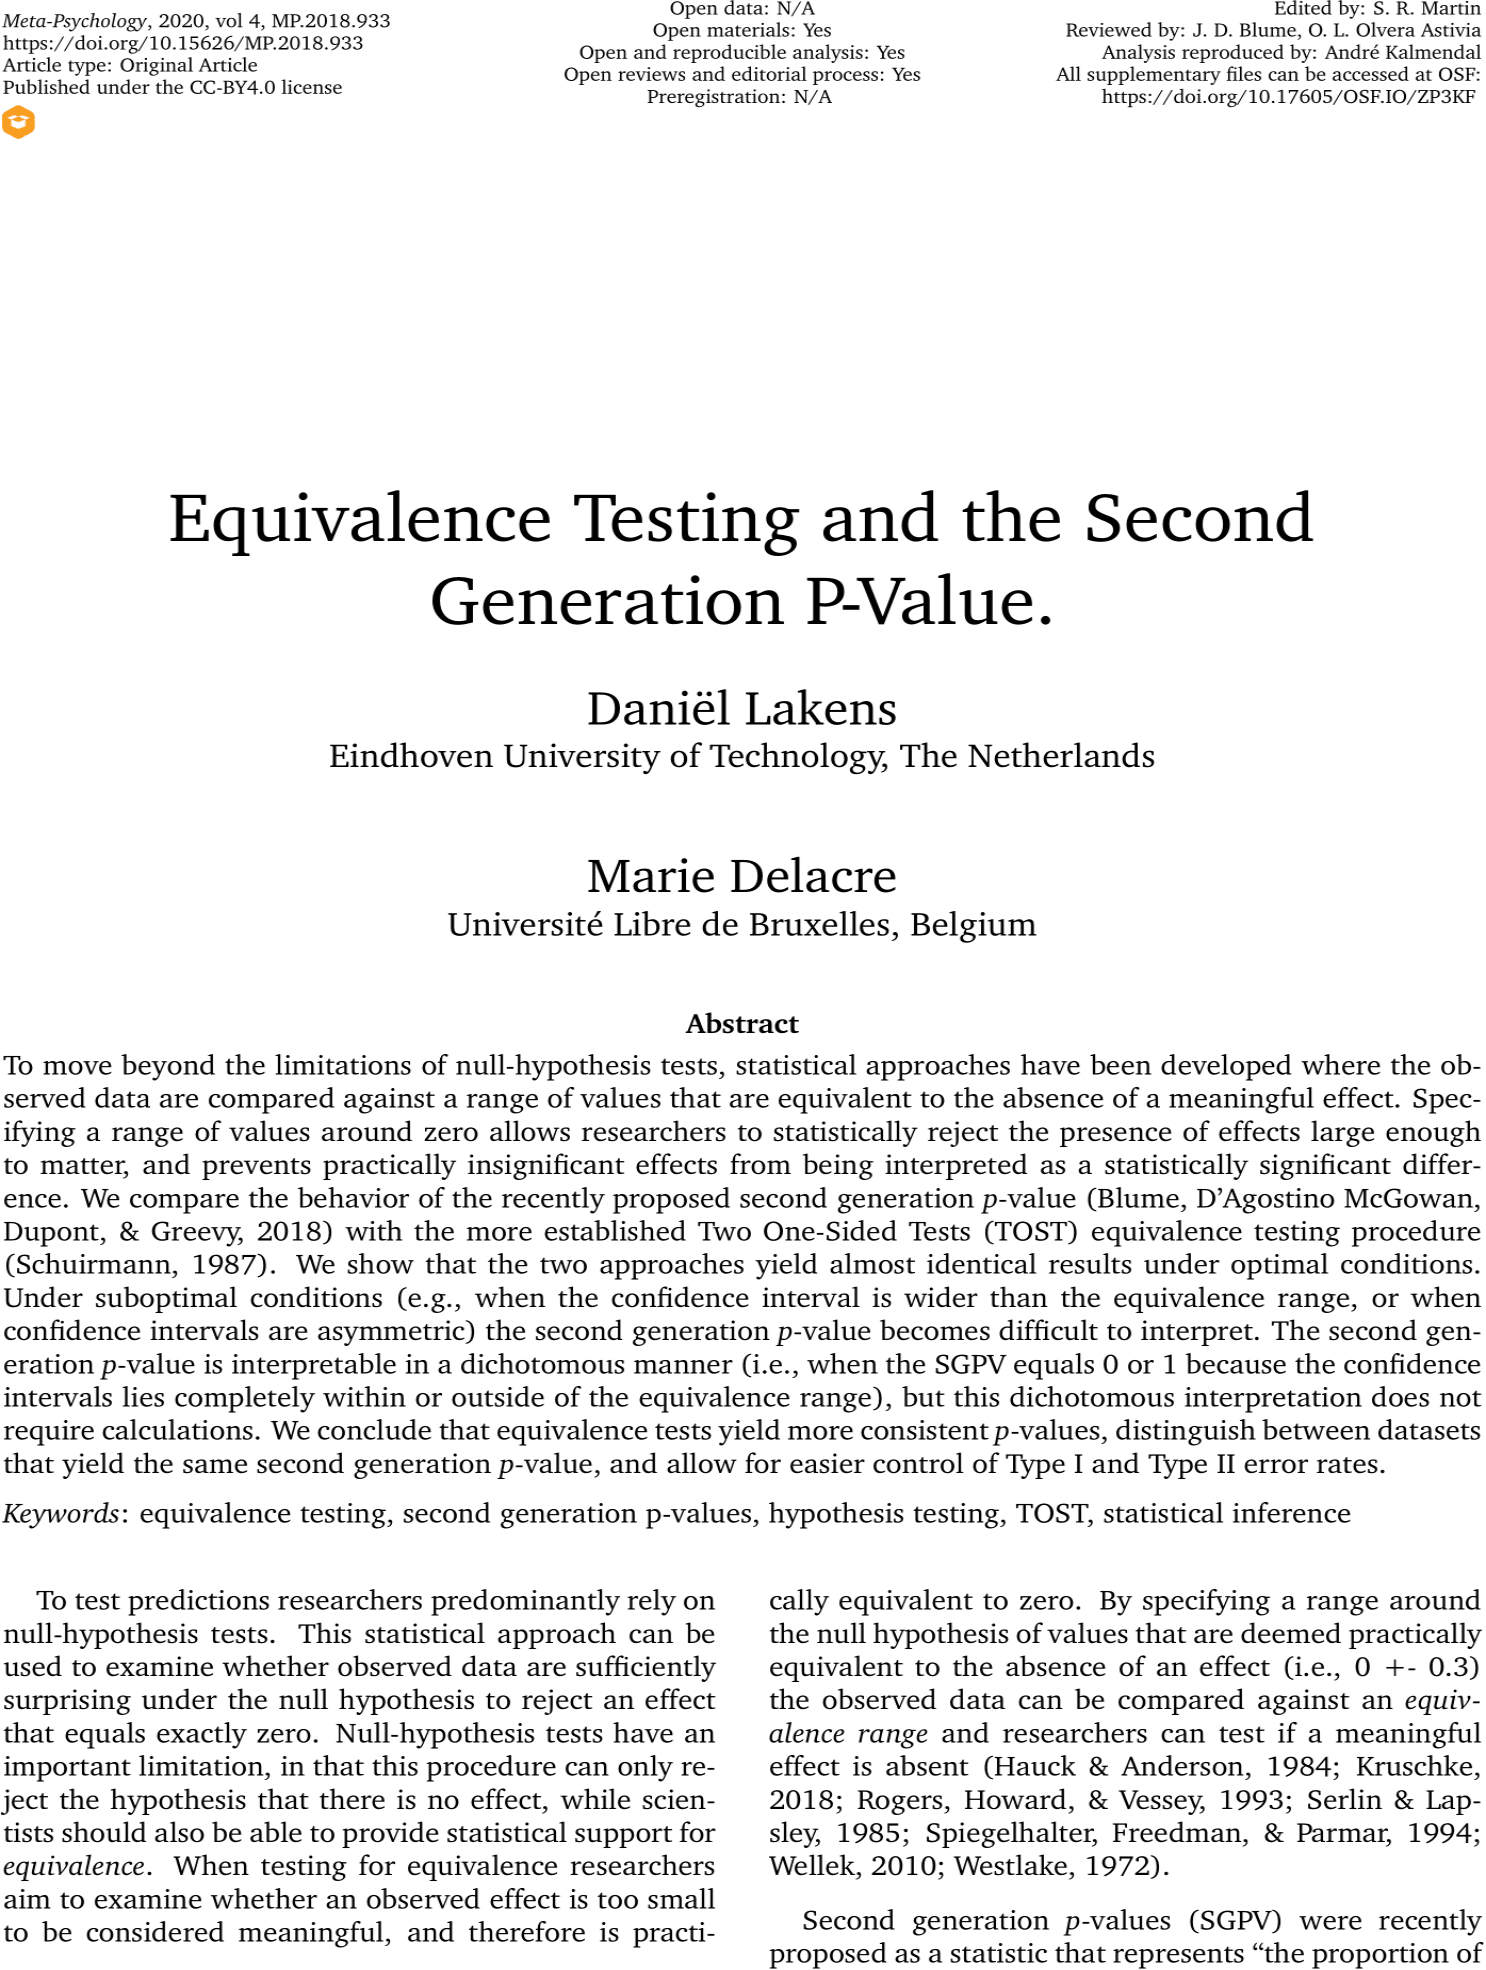
\includegraphics[width=0.92\linewidth]{D:/Documents/Github_projects/thesis/Chapitre 5/Chapitre 5-1} \end{center}

\begin{center}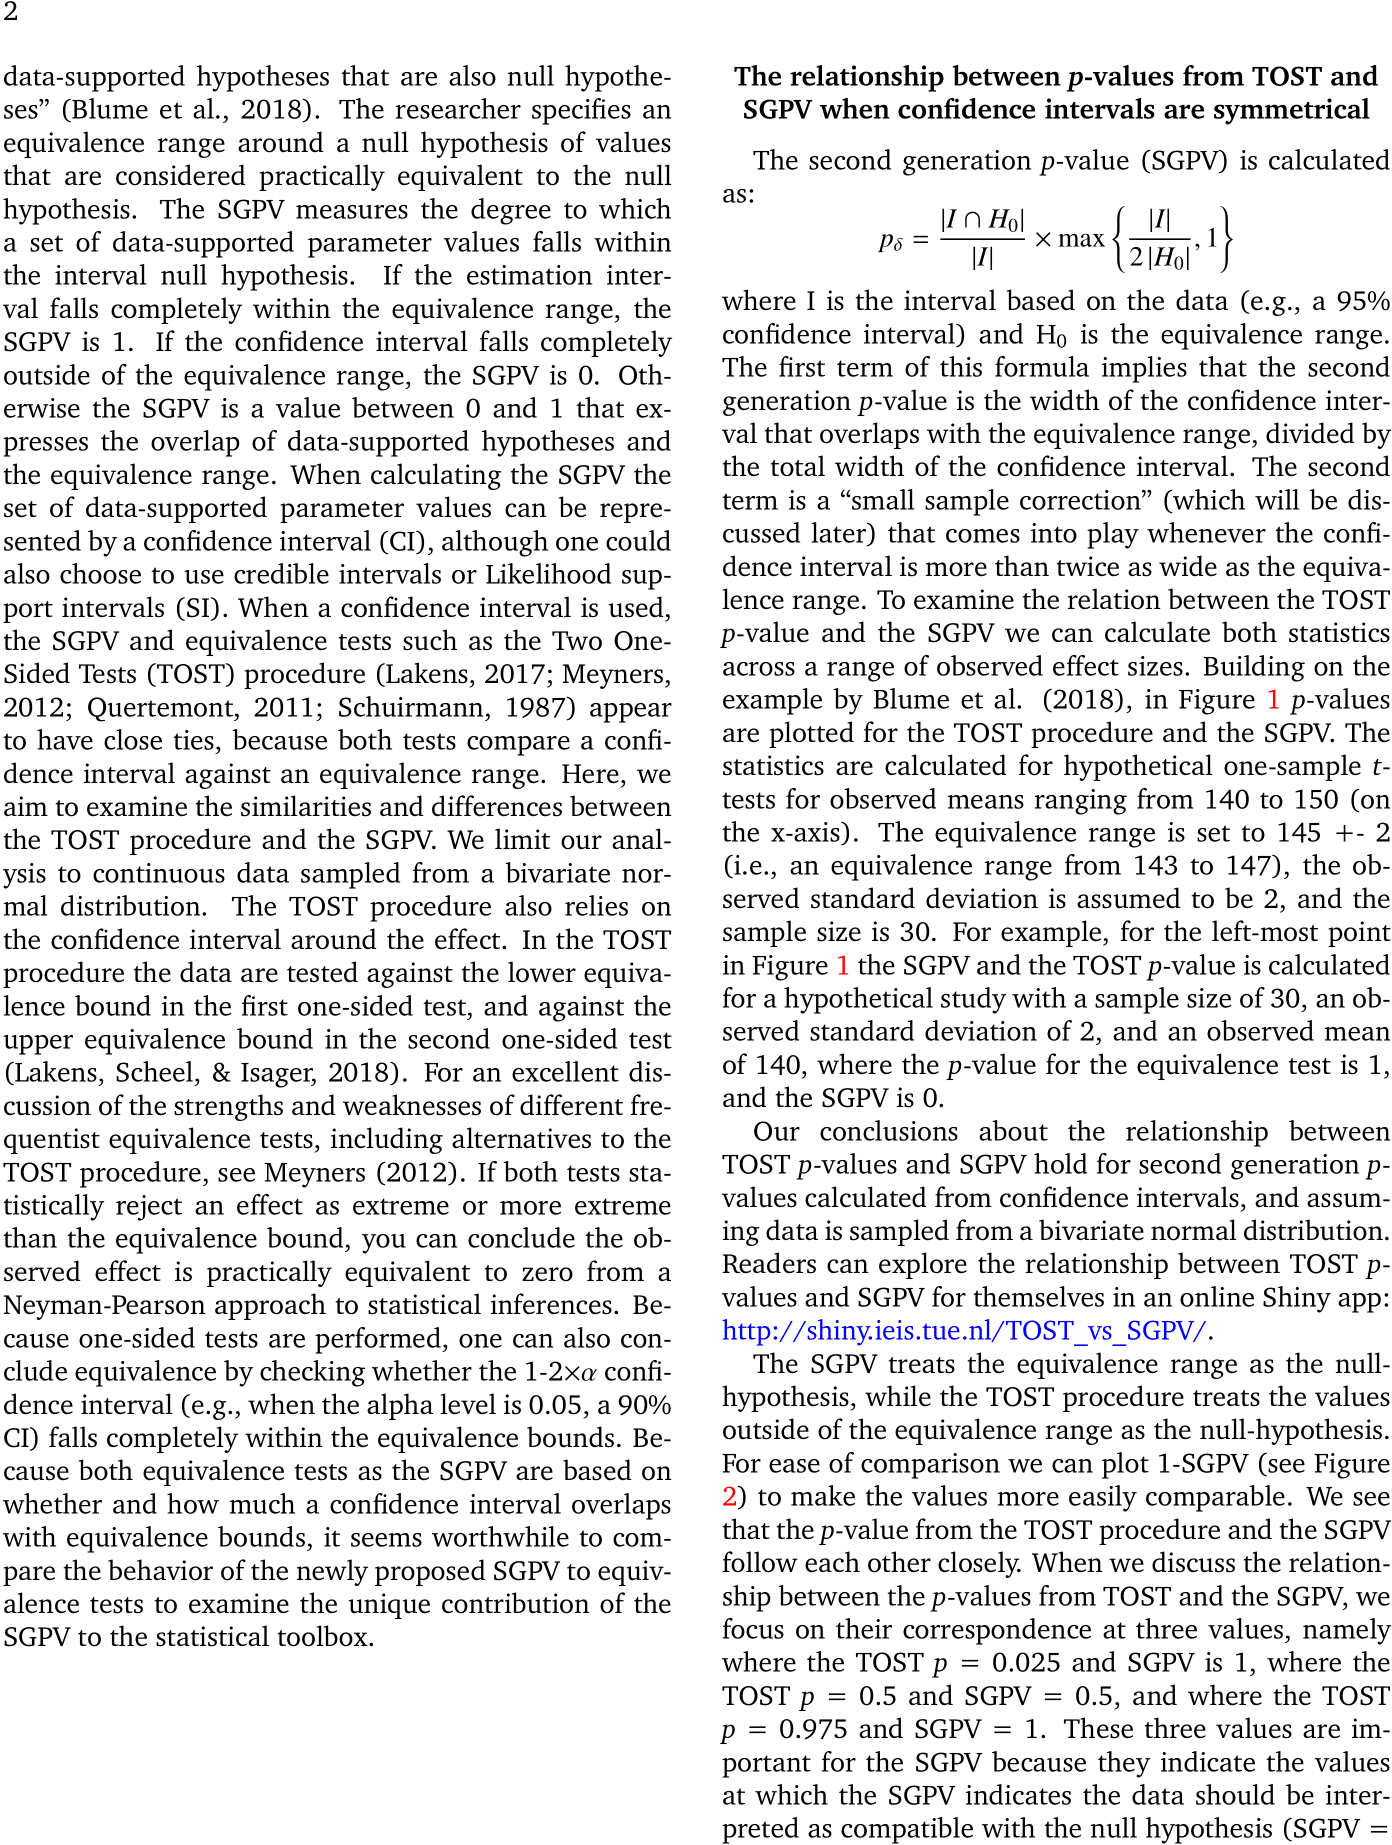
\includegraphics[width=5.51in]{D:/Documents/Github_projects/thesis/Chapitre 5/Chapitre 5-2} \end{center}

\begin{center}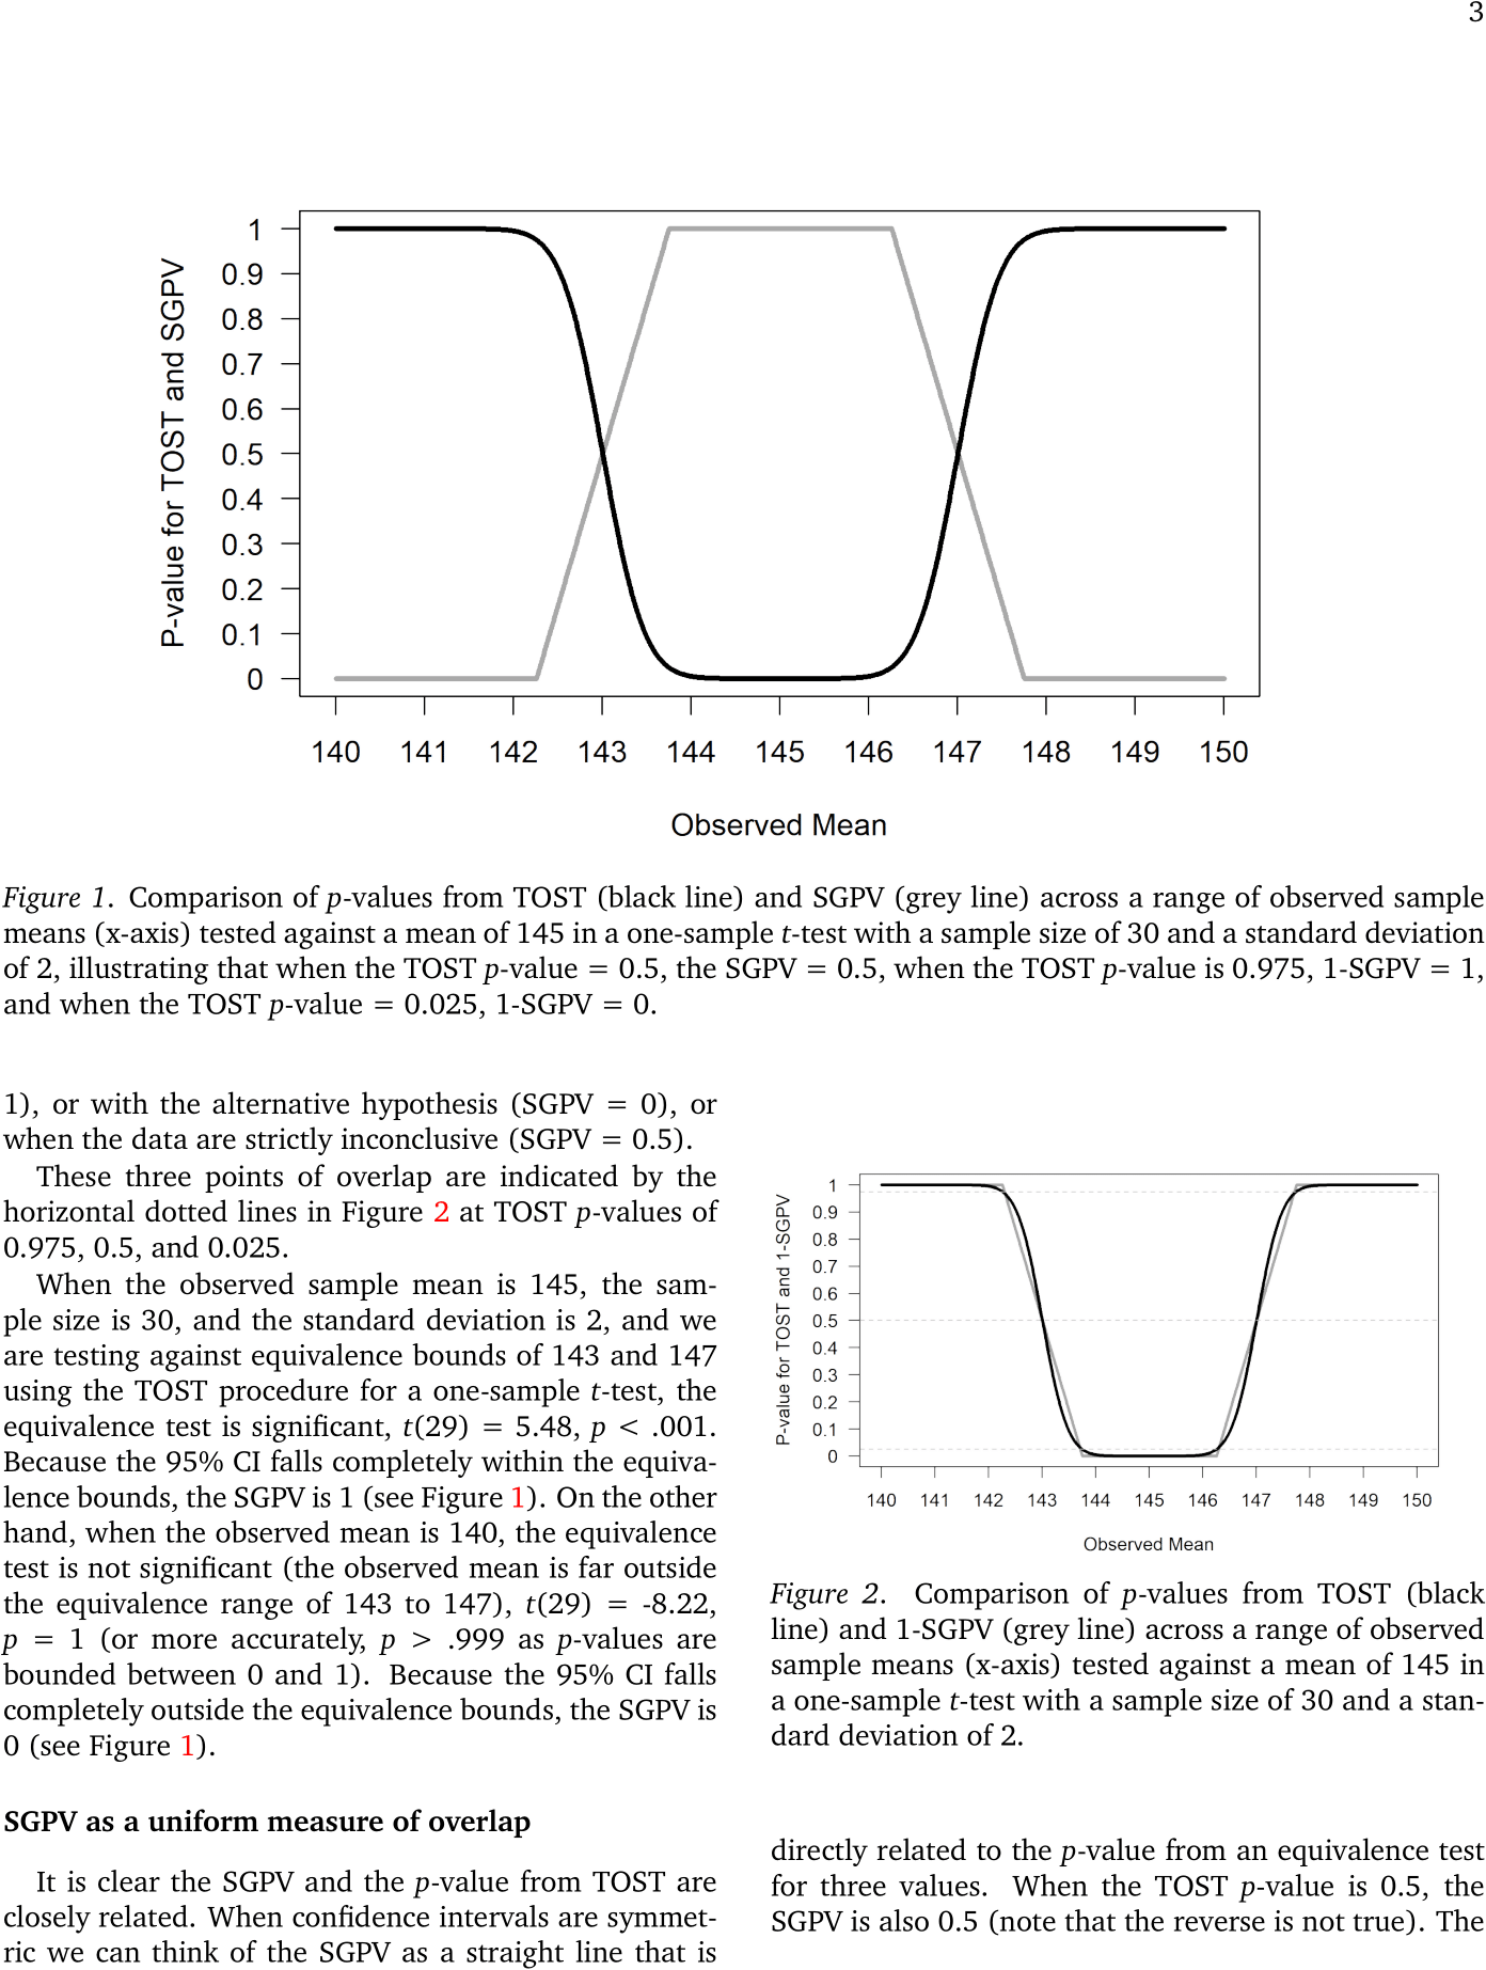
\includegraphics[width=5.51in]{D:/Documents/Github_projects/thesis/Chapitre 5/Chapitre 5-3} \end{center}

\begin{center}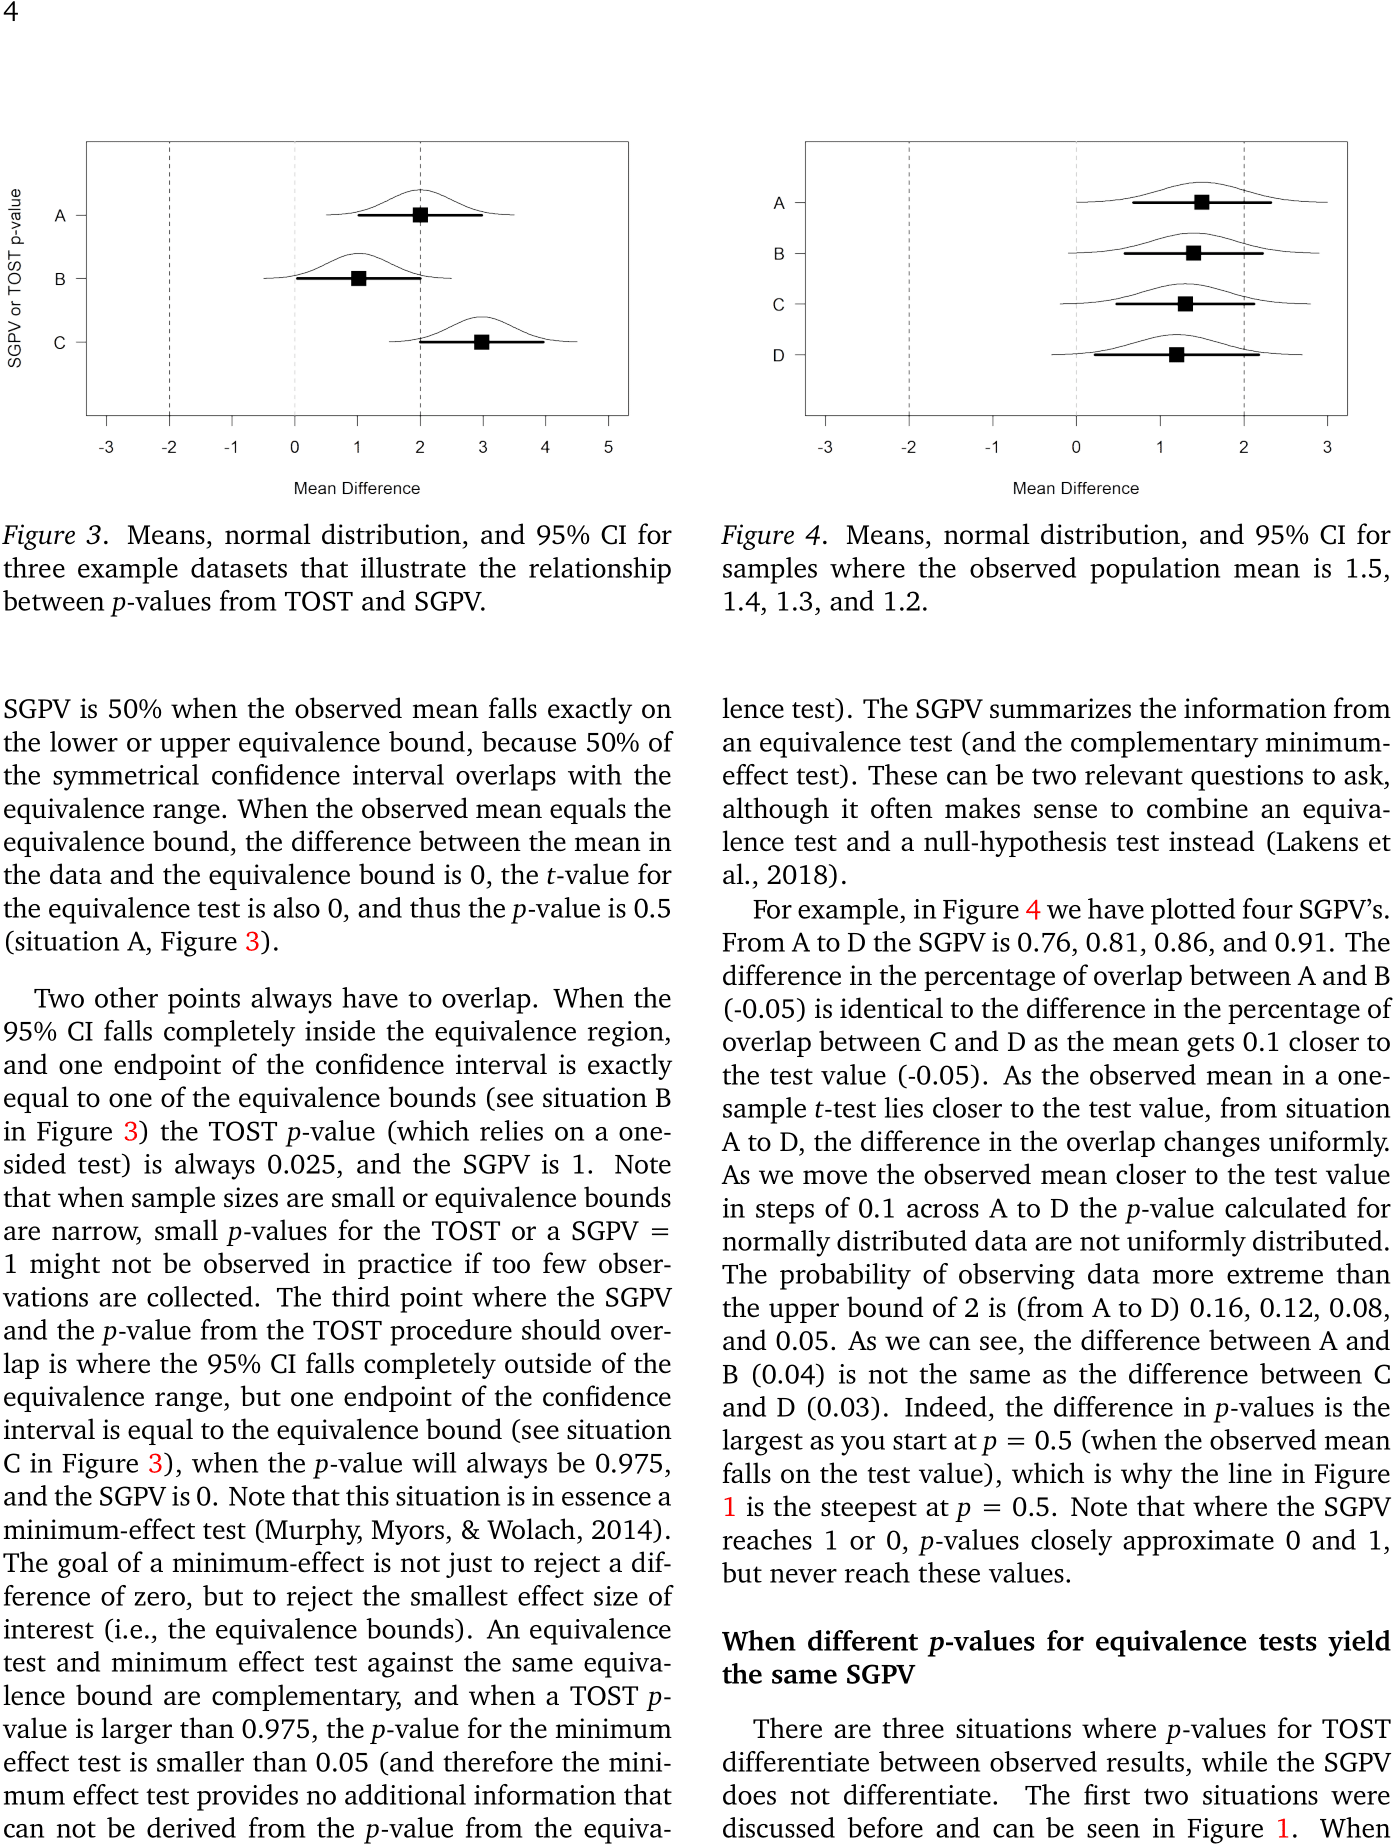
\includegraphics[width=5.51in]{D:/Documents/Github_projects/thesis/Chapitre 5/Chapitre 5-4} \end{center}

\begin{center}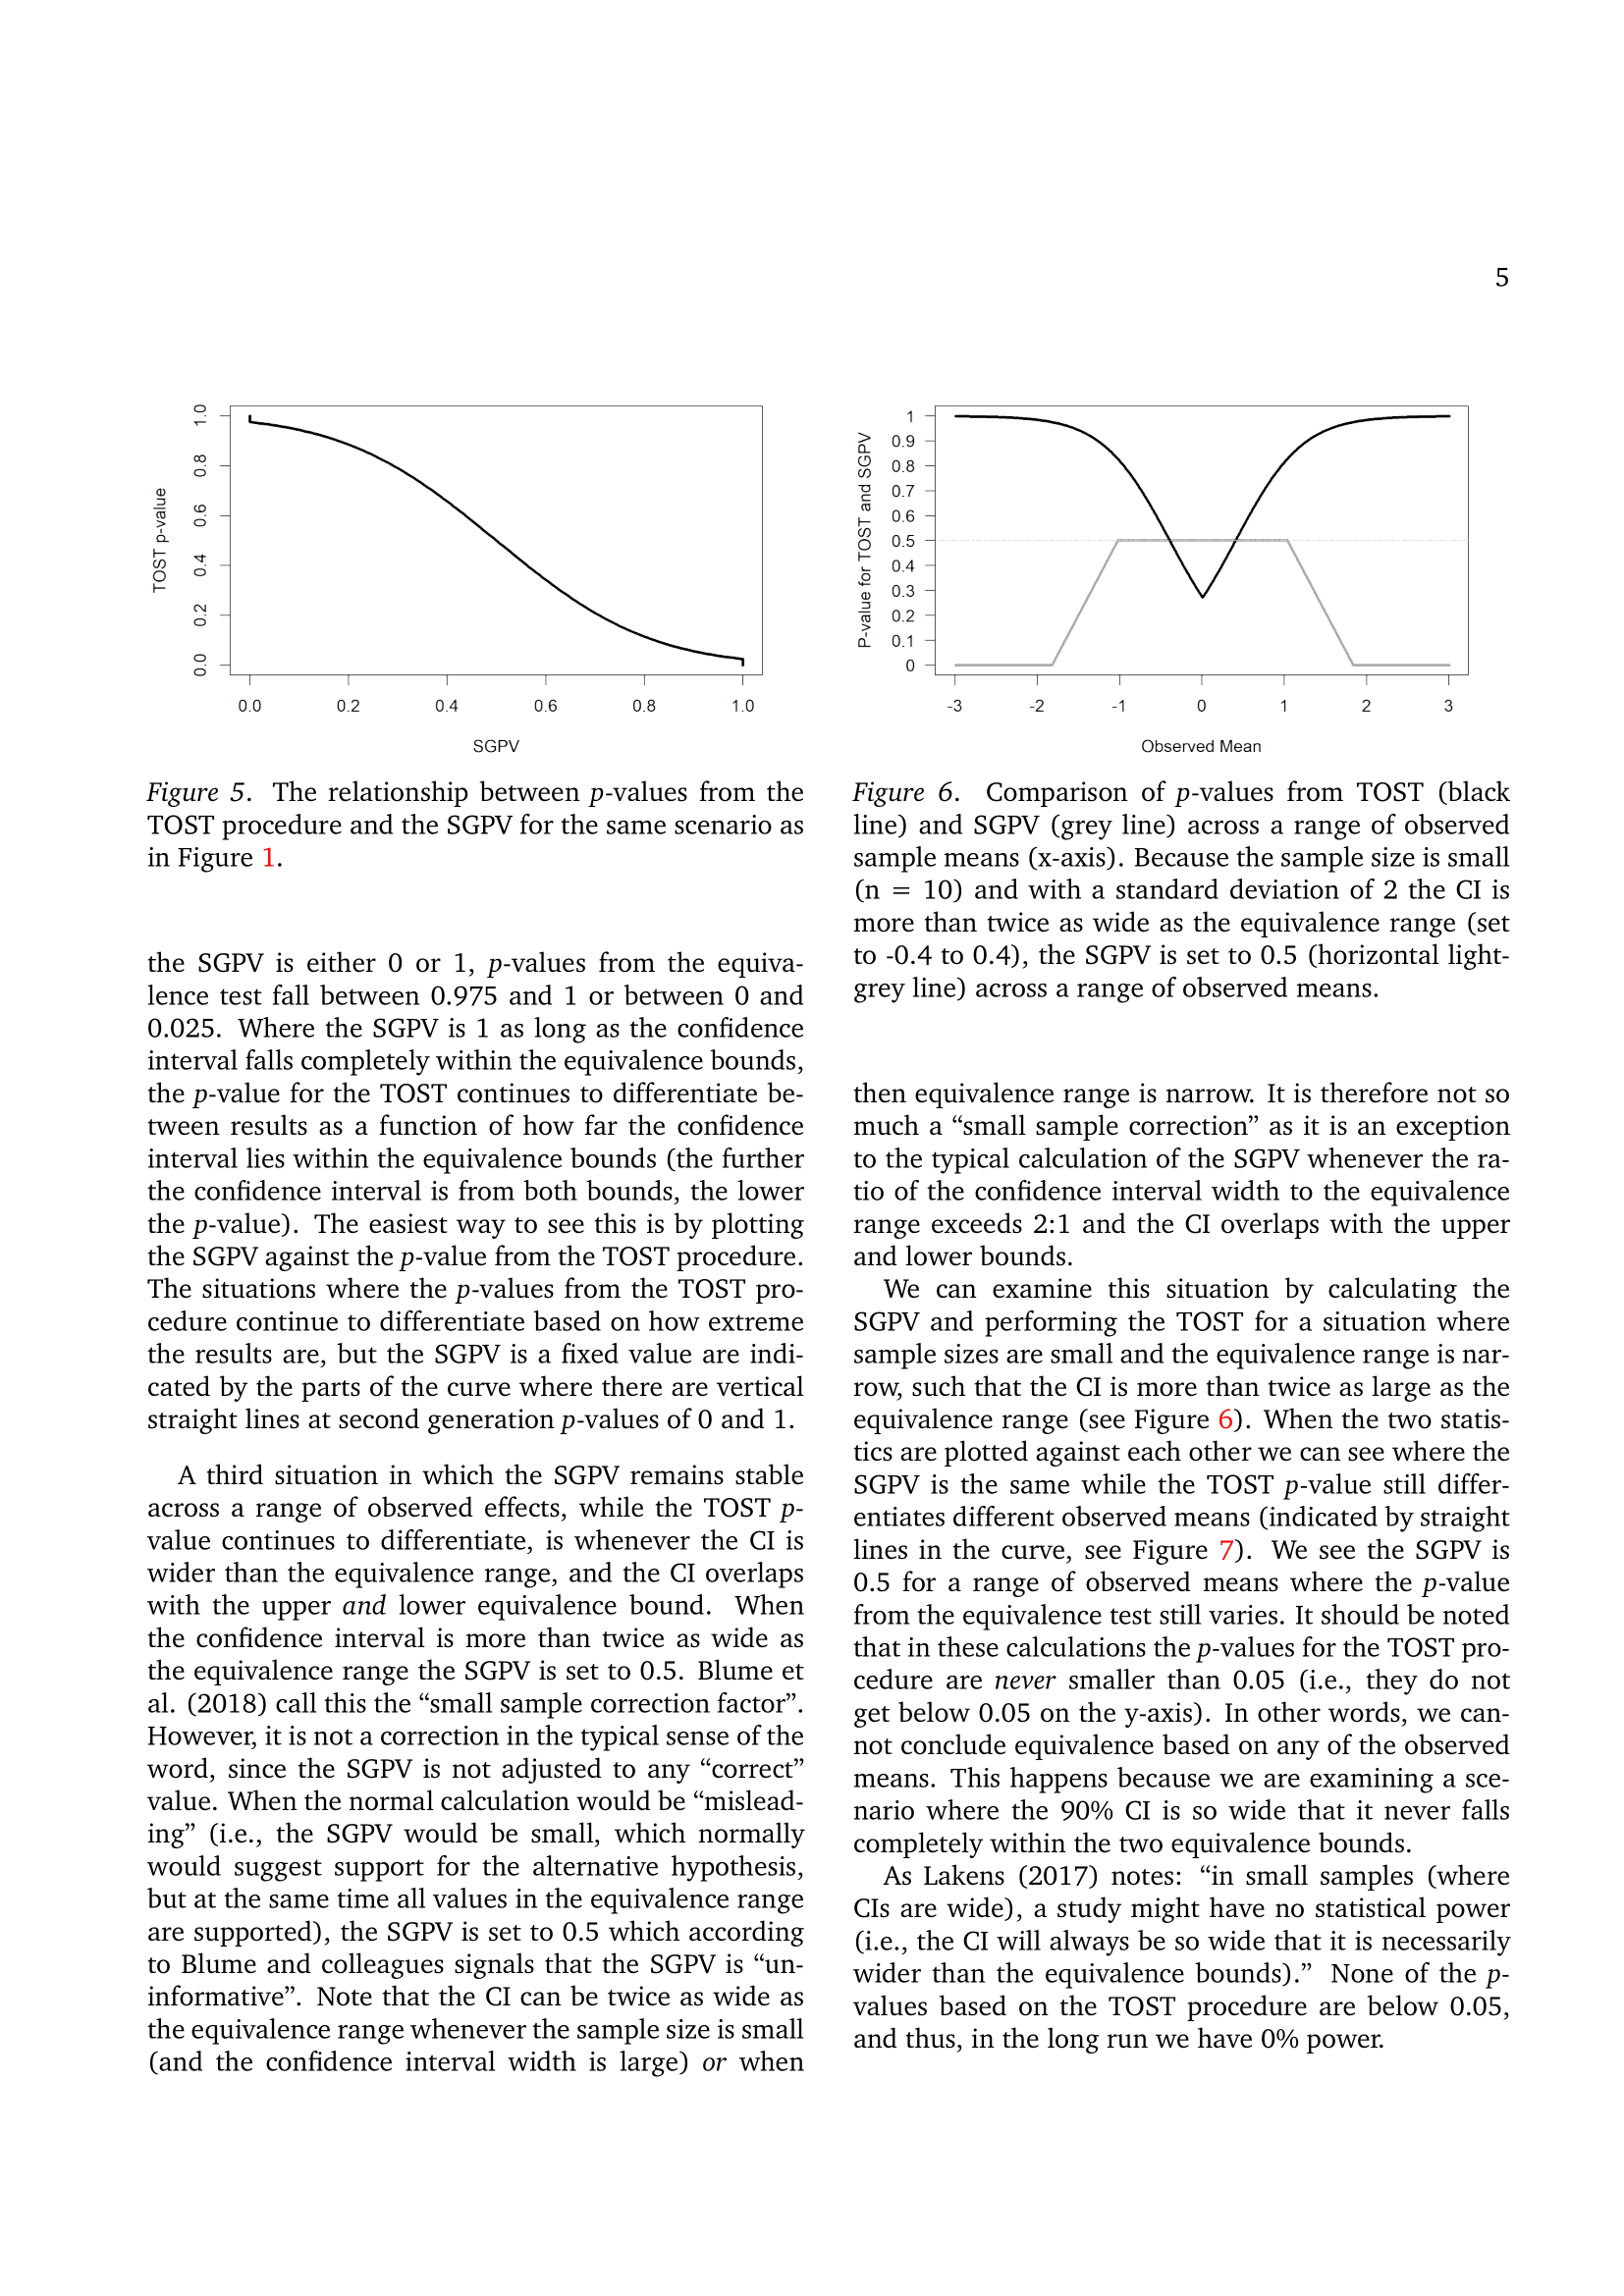
\includegraphics[width=5.51in]{D:/Documents/Github_projects/thesis/Chapitre 5/Chapitre 5-5} \end{center}

\begin{center}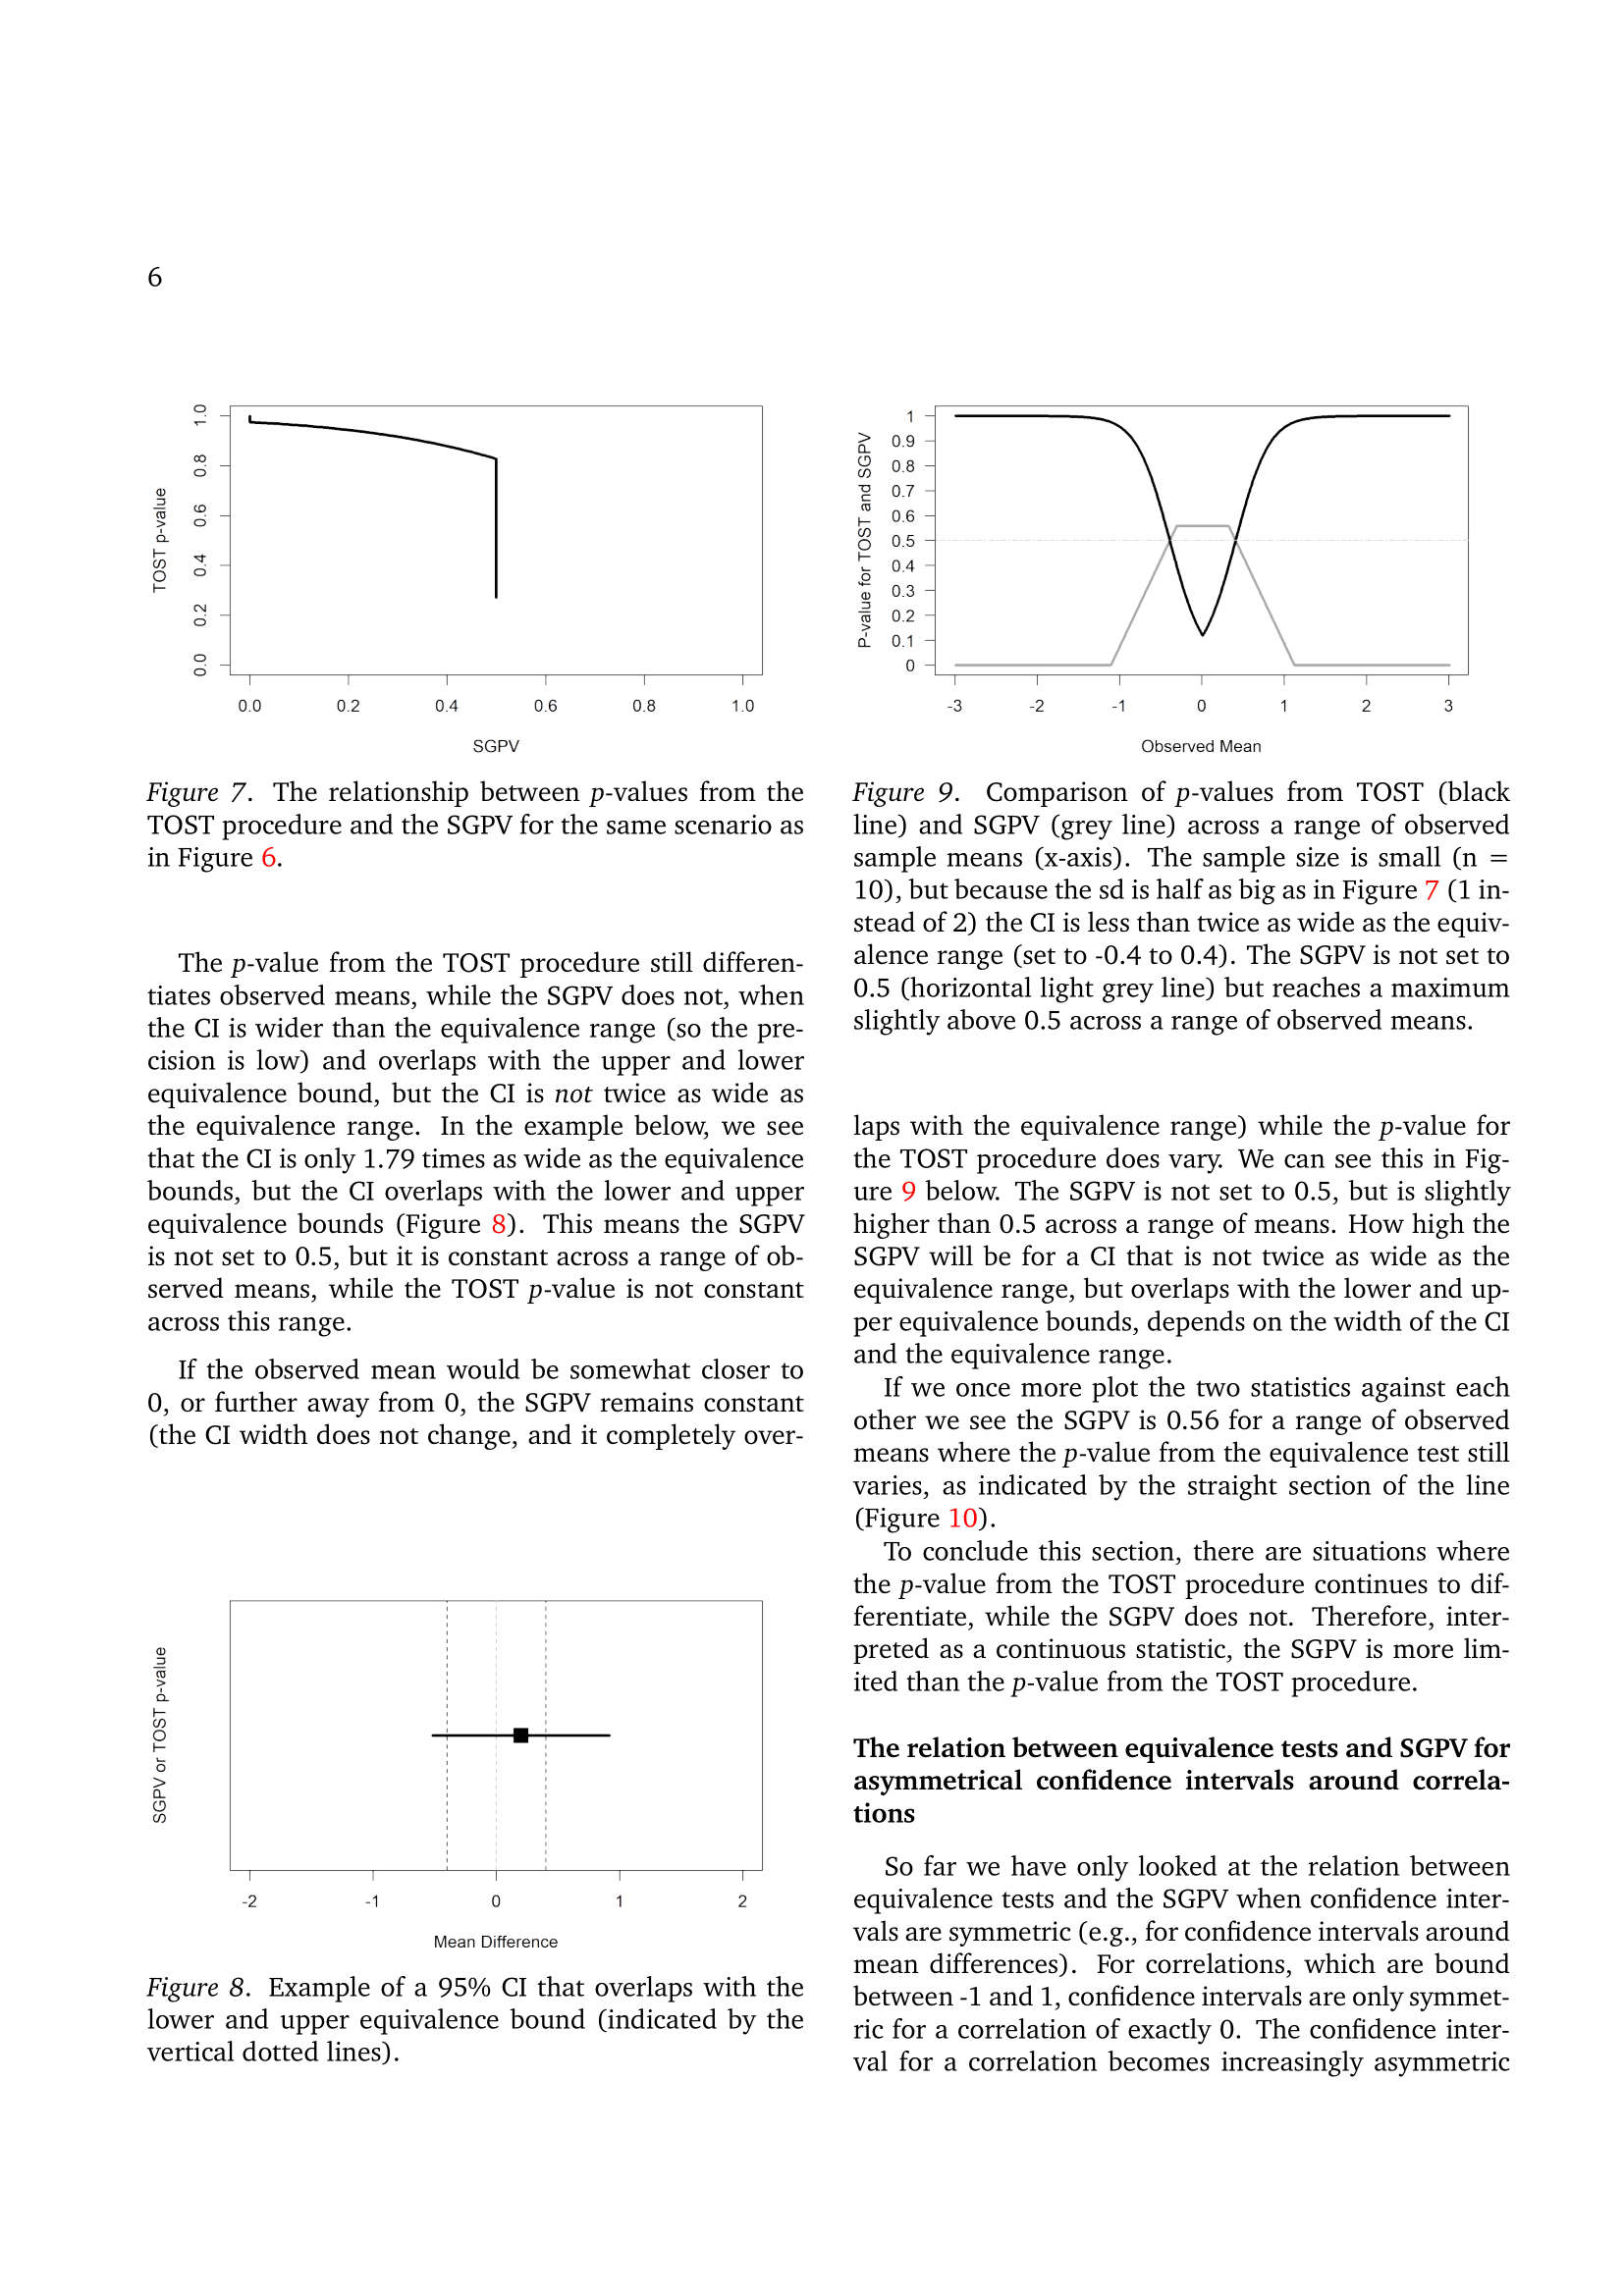
\includegraphics[width=5.51in]{D:/Documents/Github_projects/thesis/Chapitre 5/Chapitre 5-6} \end{center}

\begin{center}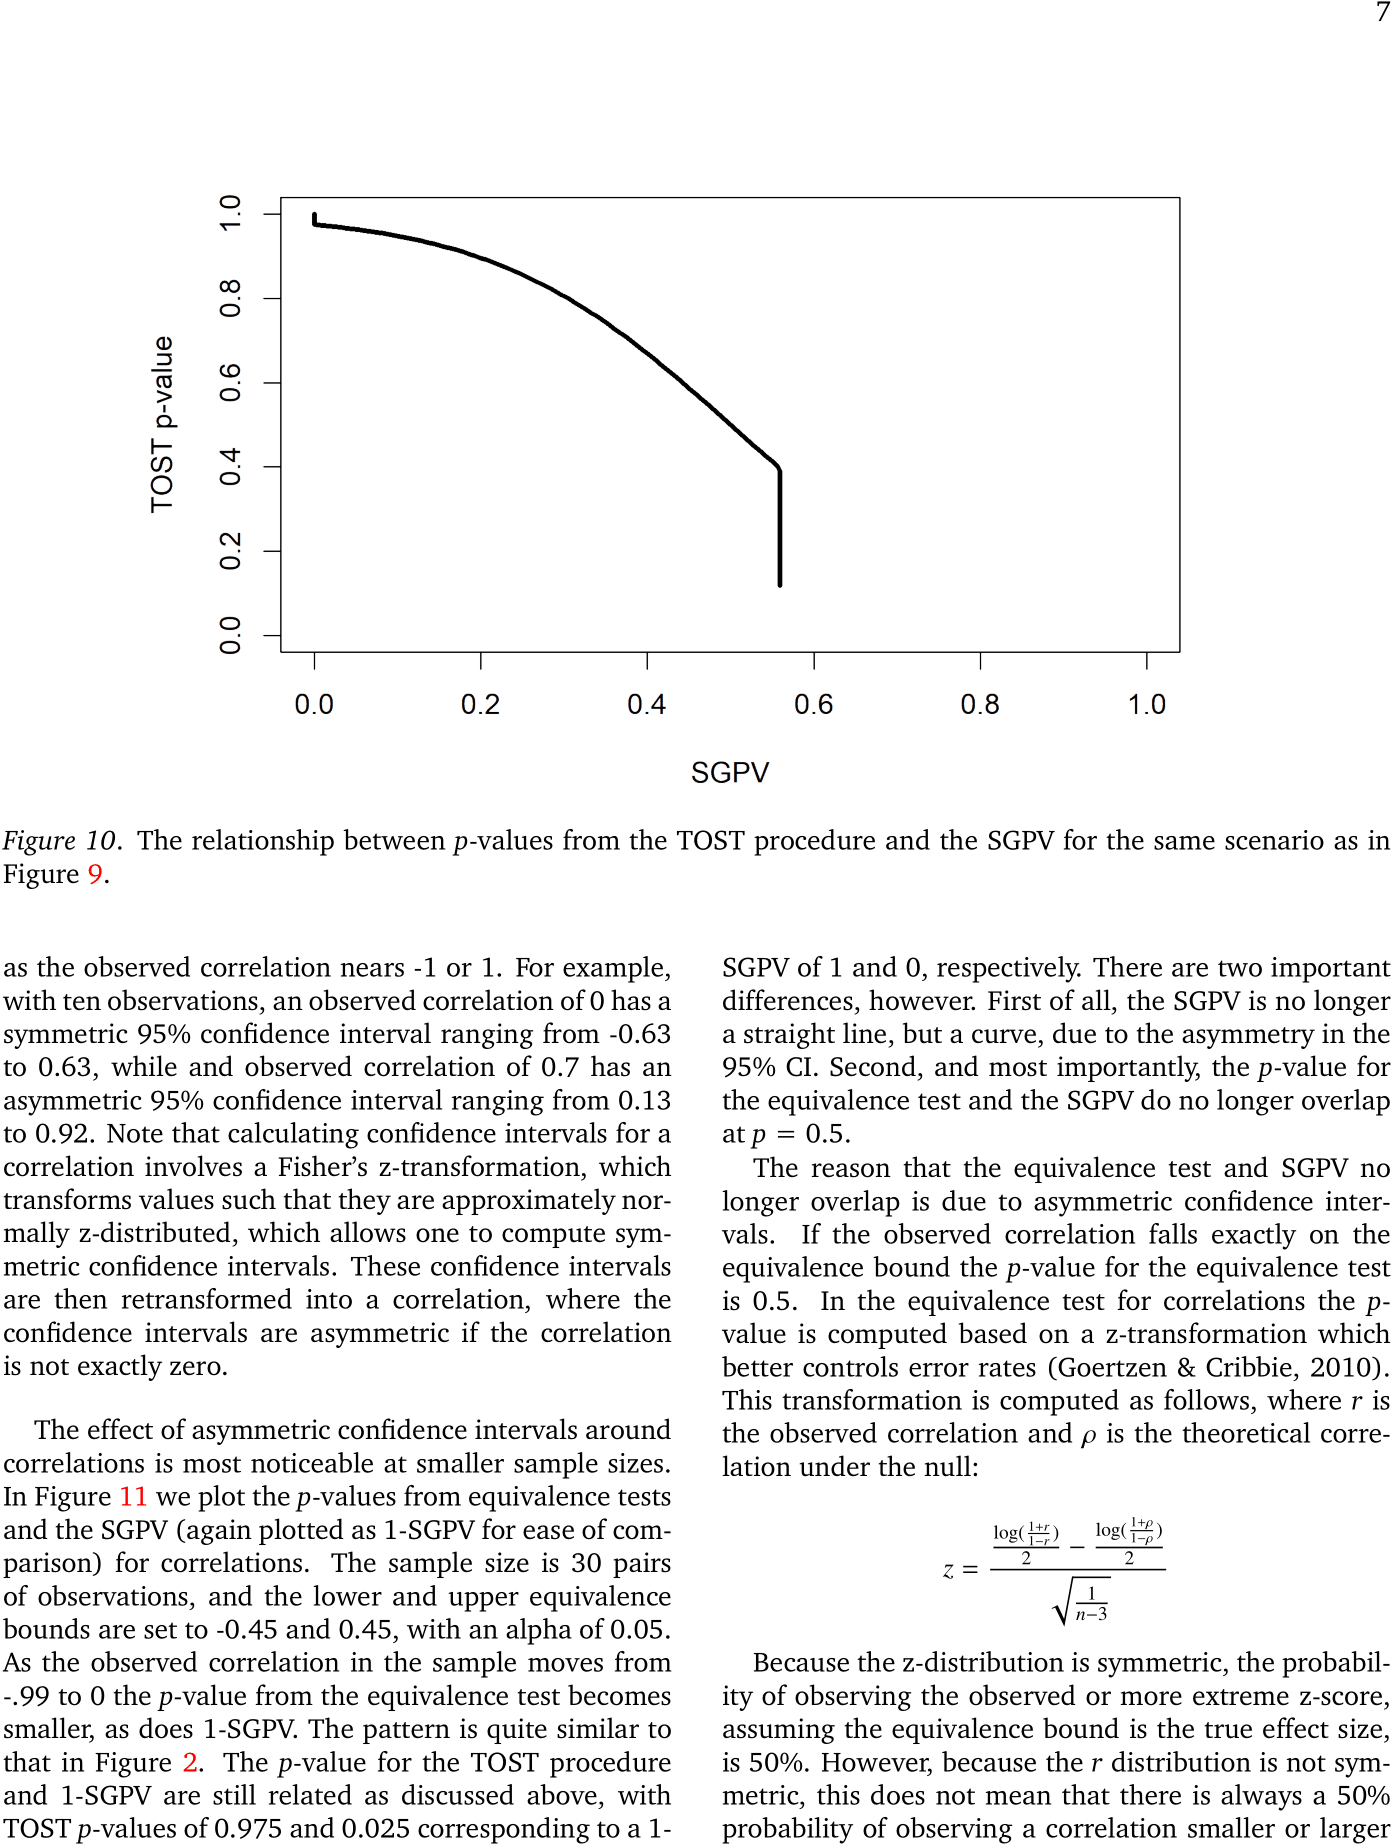
\includegraphics[width=5.51in]{D:/Documents/Github_projects/thesis/Chapitre 5/Chapitre 5-7} \end{center}

\begin{center}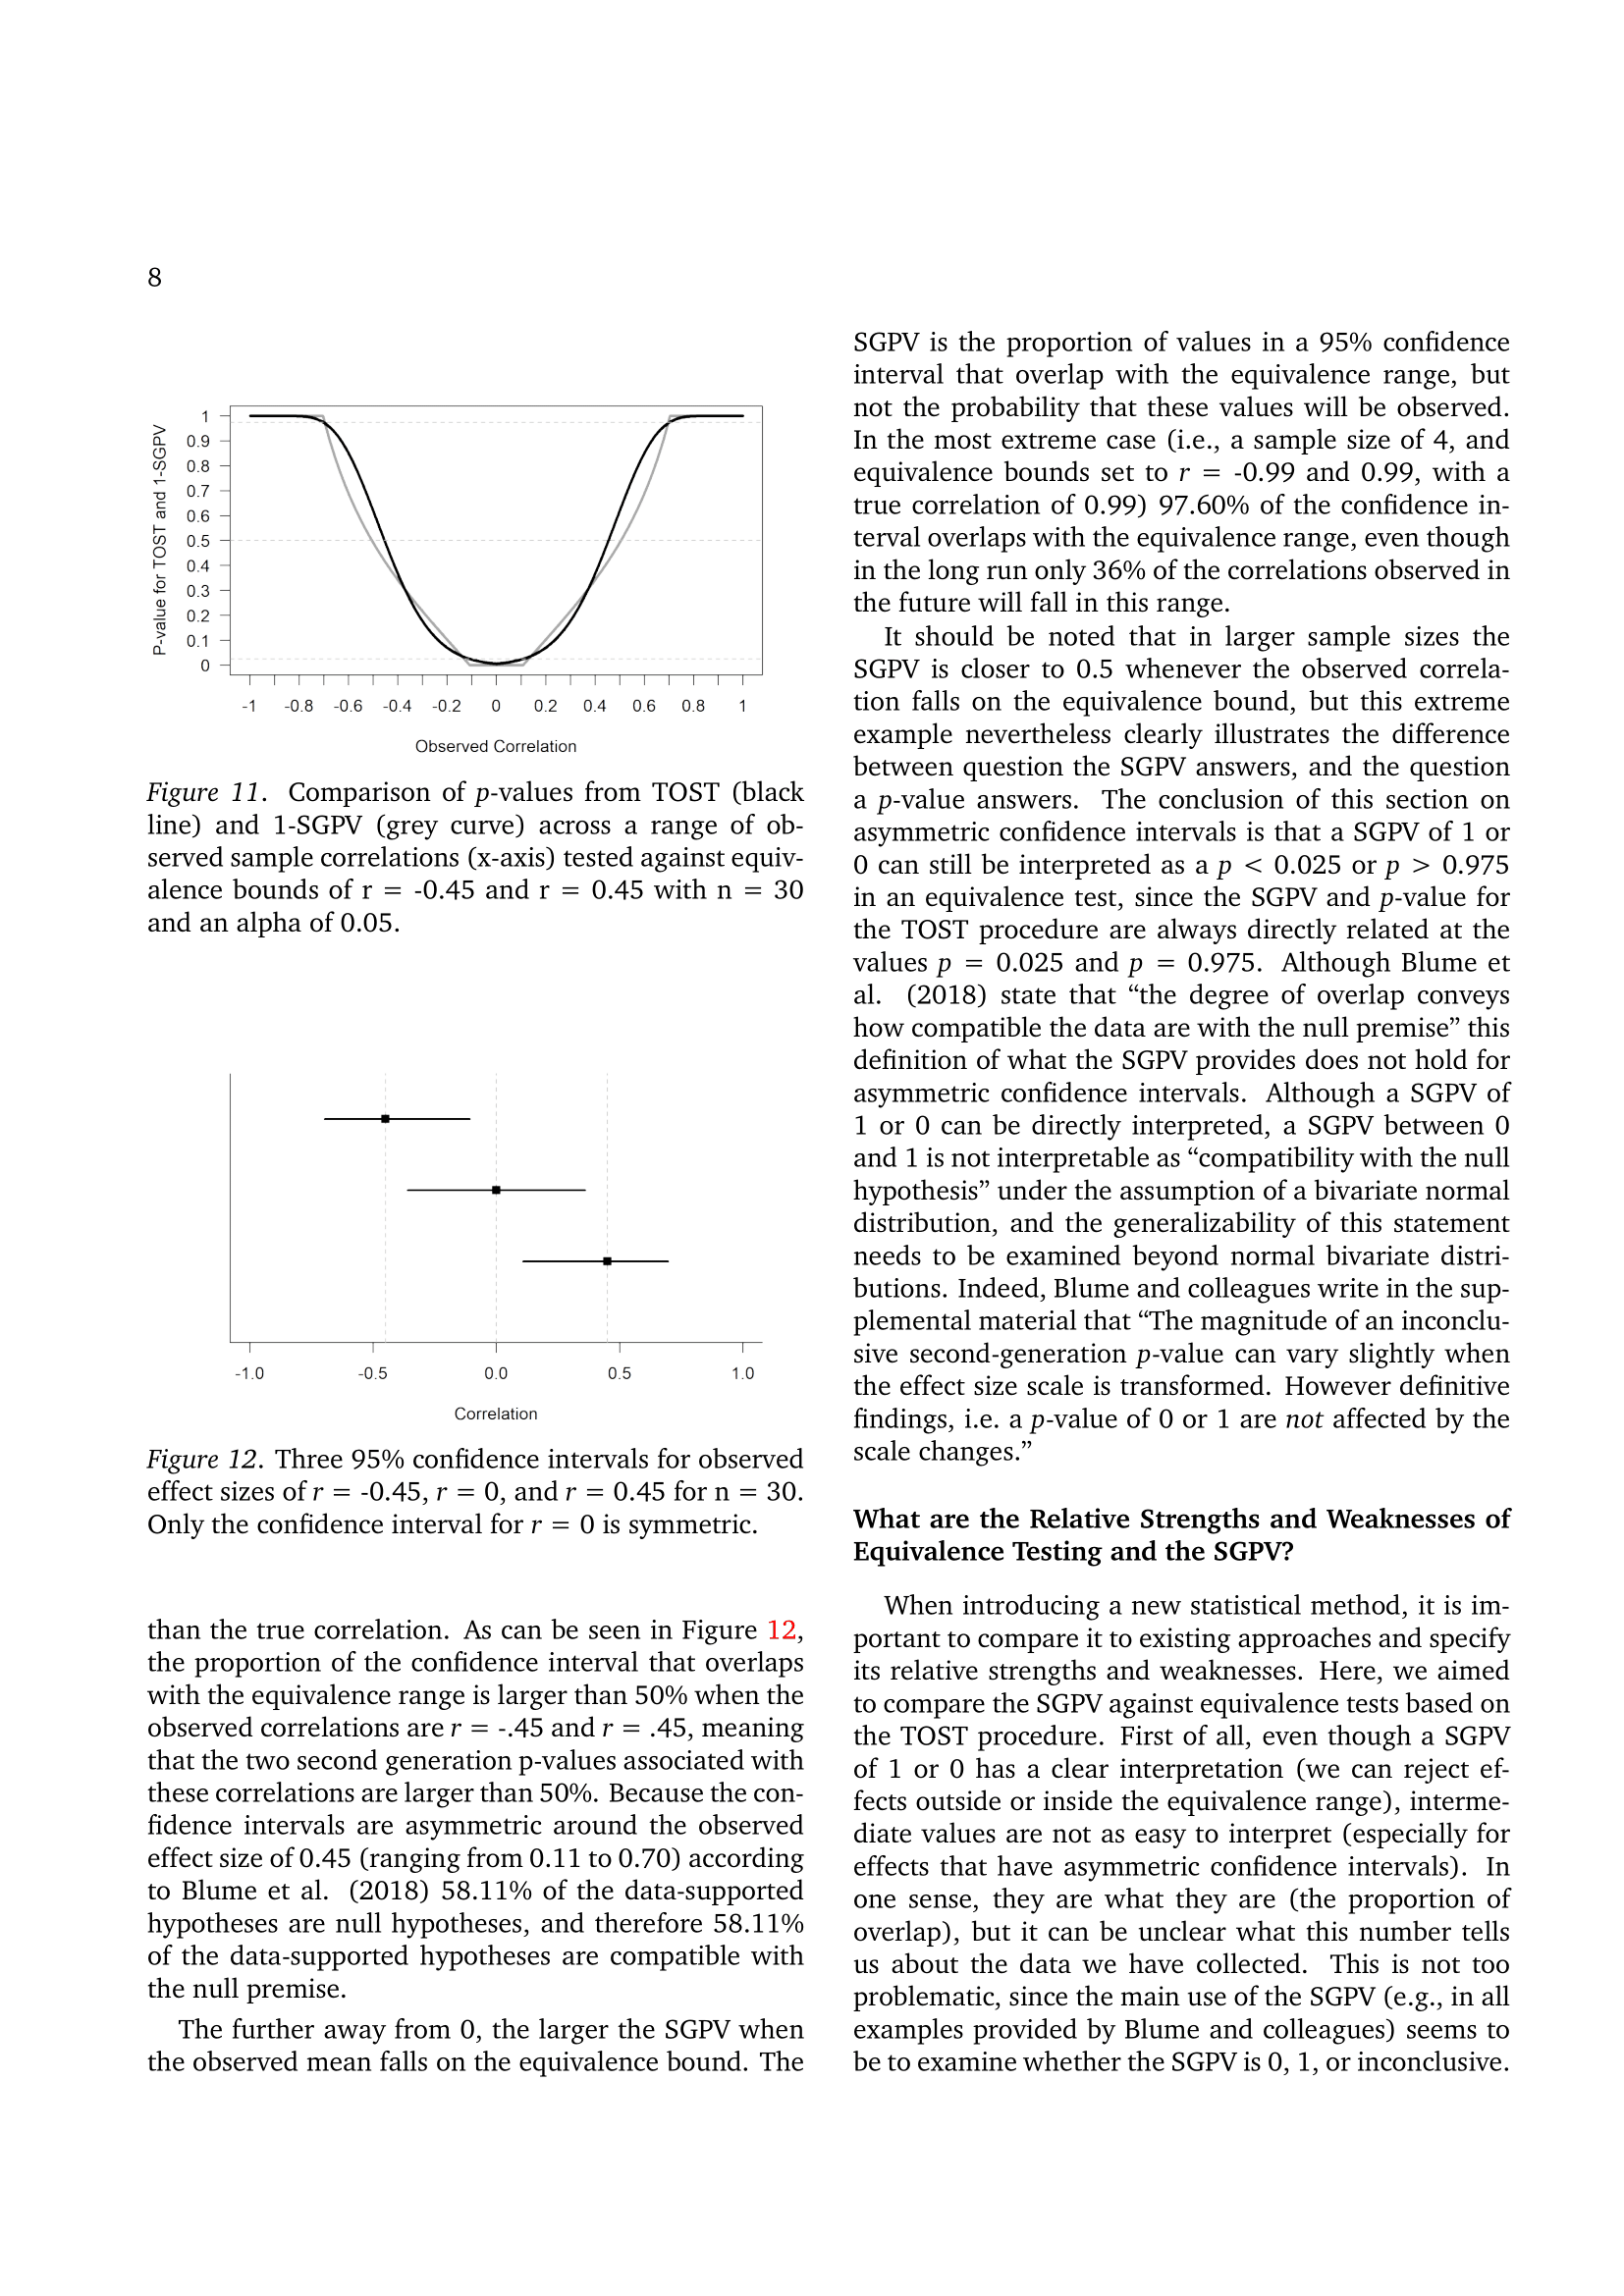
\includegraphics[width=5.51in]{D:/Documents/Github_projects/thesis/Chapitre 5/Chapitre 5-8} \end{center}

\begin{center}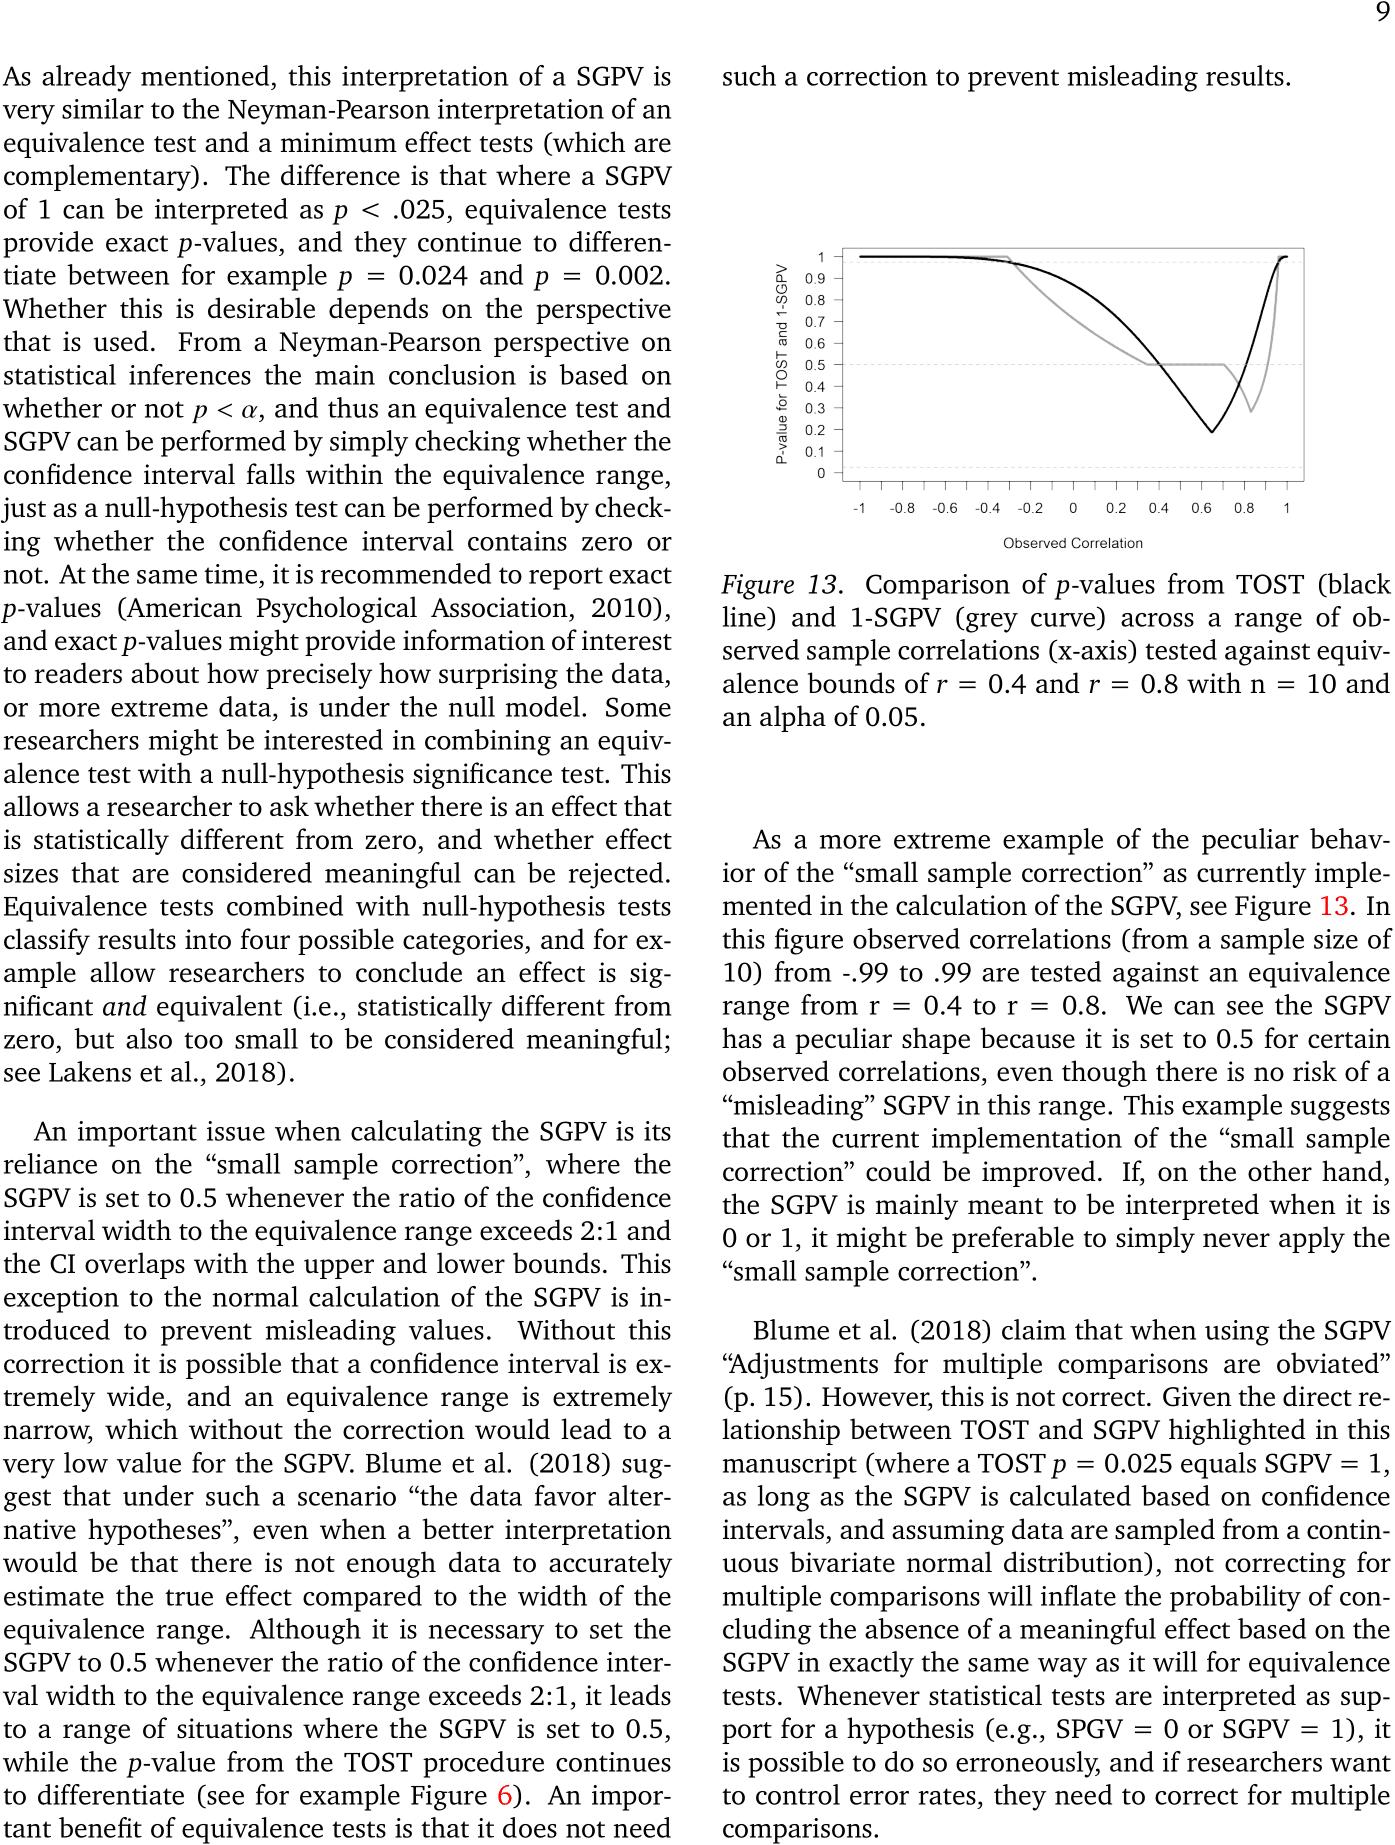
\includegraphics[width=5.51in]{D:/Documents/Github_projects/thesis/Chapitre 5/Chapitre 5-9} \end{center}

\begin{center}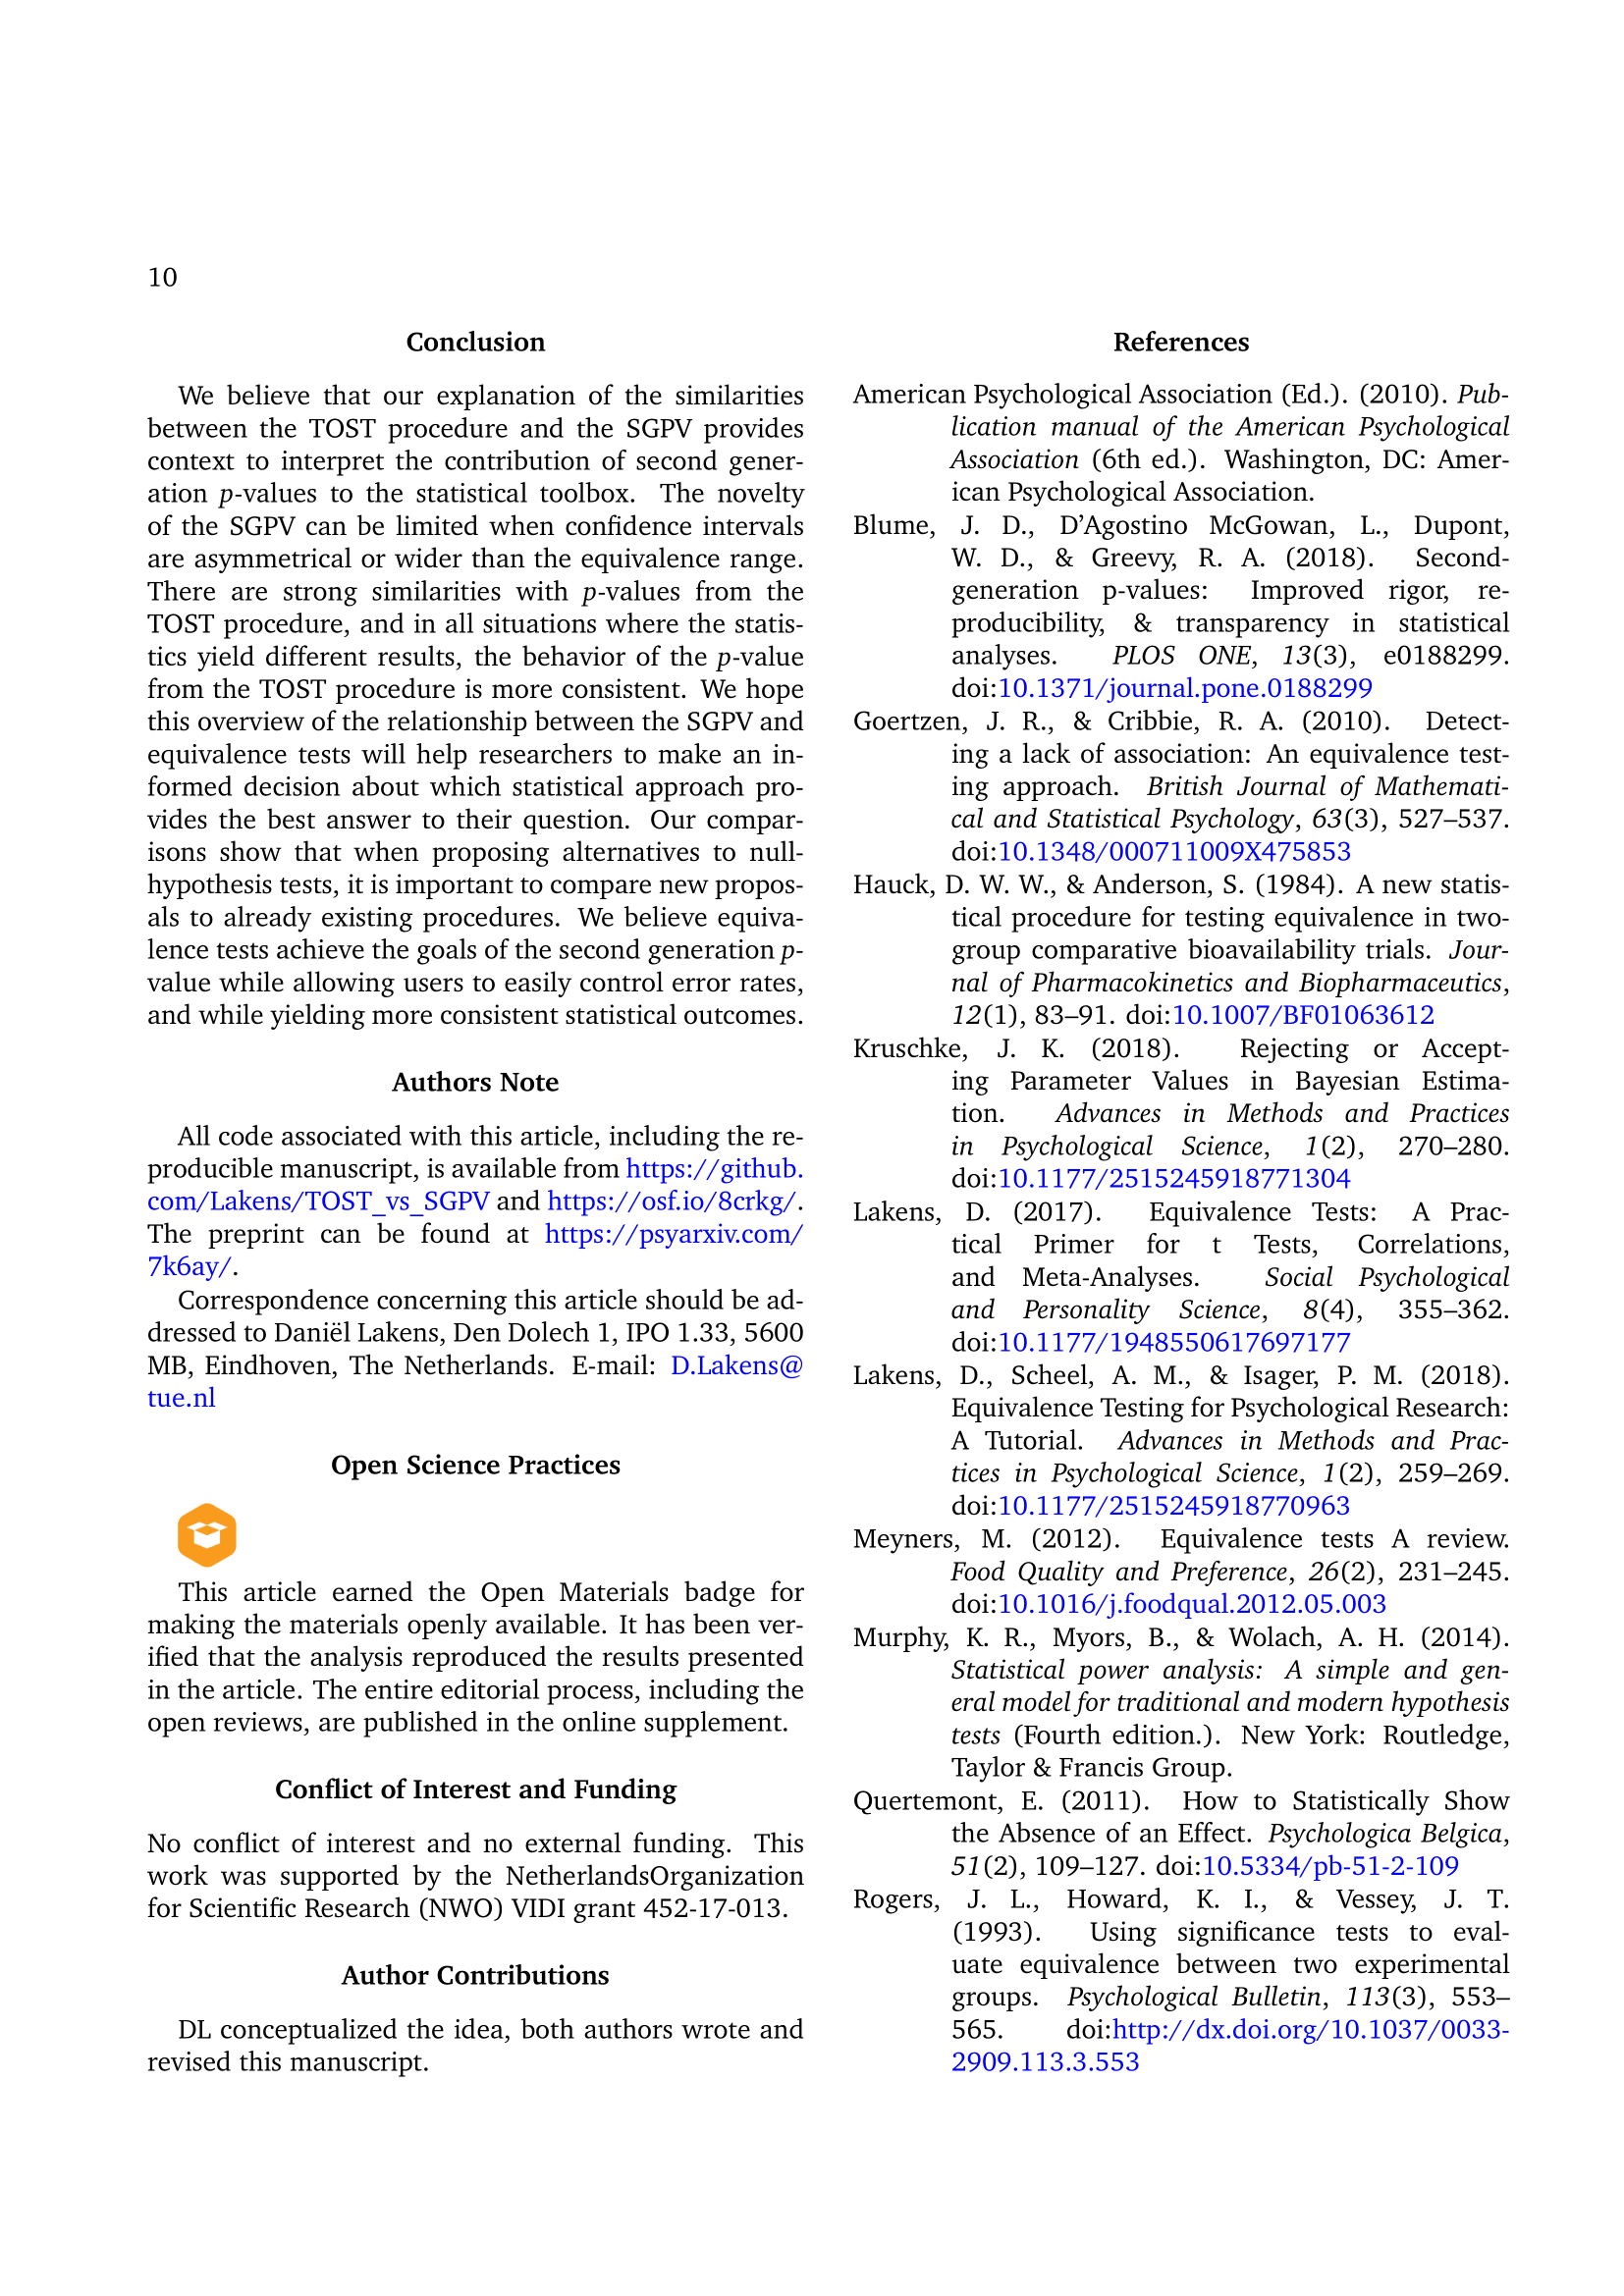
\includegraphics[width=5.51in]{D:/Documents/Github_projects/thesis/Chapitre 5/Chapitre 5-10} \end{center}

\begin{center}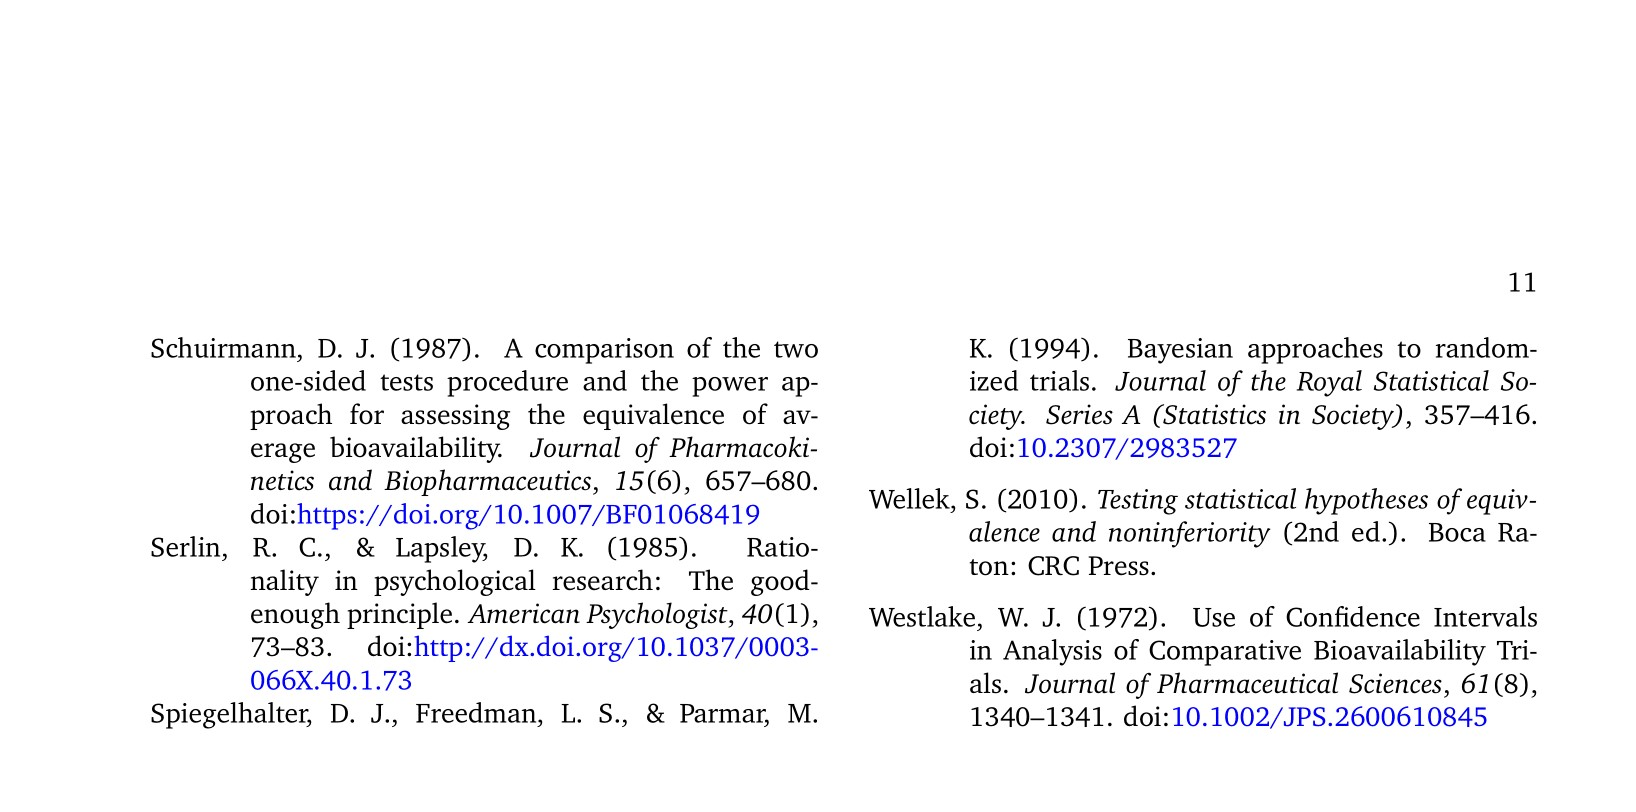
\includegraphics[width=5.51in]{D:/Documents/Github_projects/thesis/Chapitre 5/Chapitre 5-11} \end{center}


\end{document}
